%\documentclass[12pt]{article}
%\documentclass[letterpaper,amsmath,amssymb,floatfix]{revtex4}
\documentclass[preprint,notitlepage,amsmath,amssymb,floatfix]{revtex4-1}

\usepackage{amsmath}
\usepackage{amsfonts}
\usepackage{amssymb}
\usepackage{amsthm}
\usepackage{appendix}
\usepackage{commath}
\usepackage{mathtools}
\usepackage[usenames,dvipsnames]{color}
\usepackage{comment}
\usepackage{enumitem}
\usepackage{float}
\usepackage[top=1in, bottom=1in, left=1in, right=1in]{geometry}
\usepackage{graphicx}
\usepackage{listings}
\usepackage{silence}
\usepackage{tabto}

\DeclareMathOperator{\sech}{sech}

\definecolor{OliveGreen}{cmyk}{0.64,0,0.95,0.40}
\definecolor{lightlightgray}{gray}{0.9}

\TabPositions{2cm}

\WarningFilter{revtex4-1}{Repair the float}

\newcommand{\XXX}[3]{{\bf [#1: } {\tt #3} {\it -#2-}{\bf ]}}

\begin{document}

\title{Causal Set Research Notes}

\author{Will Cunningham}

\affiliation{Northeastern University}
\collaboration{Krioukov Research Group}
\noaffiliation

\date{\today}

\lstset{
language=C,
basicstyle=\ttfamily,
keywordstyle=\color{OliveGreen},
commentstyle=\color{gray},
%numbers=left,
%numberstyle=\tiny,
%stepnumber=1,
%numbersep=5pt,
backgroundcolor=\color{lightlightgray},
frame=none,
tabsize=2,
captionpos=b,
breaklines=true,
breakatwhitespace=false,
showspaces=false,
showtabs=false,
columns=flexible,
morekeywords={__global__, __device__, __shared__, threadIdx, blockIdx, blockDim, float4},
}

\maketitle

\tableofcontents

\newpage

%%%%%%%%%%
\begin{abstract}
This project is a continuation of the work described in~\cite{ref:nc2012}.  
We hypothesize that a spacetime with only dark energy has a structure which may be described by discrete events uniformly distributed across a de Sitter manifold.  
Two events are connected if they share a causal relation - i.e. they lie within each other's light cones.  
A positive cosmological constant $\Lambda$ in Einstein's field equations - which corresponds to a positive dark energy density - results in a solution described by a de Sitter manifold.
When we add matter in the form of uniformly distributed dust, a singularity (or Big Bang) emerges naturally while the structure at late times remains the same.  
This connects the hubs of the networks, which are recognized as the earliest events.
Subsequently this allows us to construct a complex network with physical properties which match those of our universe, as well as mathematical properties which match those of other well-studied complex networks. \par
%%%%%%%%%%
The rescaled degree distributions for the pure-energy causal set have been previously studied in~\cite{ref:nc2012}.
In this project we compare them to the same distributions for a universe with matter over a range of physical parameters, including the ratio of matter to dark energy.
We go further to study the clustering, connectedness, and navigability of our universe.
Studying navigability alone requires addressing how to measure geodesic distances:  this remains an unsolved analytical problem.
We attempt to solve this by embedding our universe in a higher spatial dimension, and we implement several validation tests to determine if this is a legitimate approach.
We also would like to address the \textit{why now} problem:  why are the matter and dark energy densities currently the same order of magnitude?
To study this we will look for special behaviors of the network when the rescaled time is set to unity.
\end{abstract}

%%%%%%%%%%
\section{Background}
%%%%%%%%%%
In recent years, experimental observations have made us increasingly certain that we live in a flat universe which is expanding at an accelerating rate.  
The $\Lambda$CDM Model has provided a robust theoretical framework for describing the cosmological evolution of our universe, though it relies on six free parameters whose origins have not yet been elucidated.
Rather than simply relinquish this issue to the anthropic principle, we aim to identify how a causal set framework might shed light on the nature of these constraints and how they may be related.
Complex networks have given insight into problems in many unrelated fields in the past decade, so it is not unreasonable to assume they could be help out here as well. \par
%%%%%%%%%%
In our work, we are interested in studying two degrees of freedom:  the sum of the baryon and dark matter density, and the dark energy density.  
The matter and energy densities both enter Einstein's equations~\eqref{eq:einstein}, so they naturally both affect the manifold on which the causal set events lie.

\begin{equation}
\label{eq:einstein}
G_{\mu\nu} + \Lambda g_{\mu\nu} = \frac{8\pi G}{c^4}T_{\mu\nu}
\end{equation}

\noindent We can instantly recognize that if these variables are free parameters, they are somehow chosen to minimize the Einstein-Hilbert action

\begin{equation}
\label{eq:EH_Action}
S = \int\!\left[\frac{c^4}{16\pi G}R+\mathcal{L}_M\right]\sqrt{-g}\, \mathrm d^4x
\end{equation}

\noindent The dark energy density is manifested in the cosmological constant

\begin{equation}
\label{eq:dark_energy_density}
\rho_\Lambda = \frac{8\pi G}{3}\Lambda
\end{equation}

\noindent Starting from a quantum field theory, with the mass fields described by the Lagrangian density $\mathcal{L}_M$ we can obtain the stress-energy tensor by applying the Euler-Lagrange equations:

\begin{equation}
\label{eq:EL_stress_energy}
T_{\mu\nu} = -2\frac{\delta\mathcal{L}_M}{\delta g^{\mu\nu}} + g_{\mu\nu}\mathcal{L}_M
\end{equation}

\noindent The matter density is then simply proportional to the first element of this tensor, $c^2\rho_M = T_{00}$. \par
%%%%%%%%%%
This implies that the properties of the complex network we are studying will be modified when these physical parameters are modified.
In turn, if certain physical properties are extremized, so must properties of the causal set.
It is our goal to search for these properties and show through variation of these parameters that there is a local (perhaps global) extremum.
Conversely, if we take the physical scenario to arise from an underlying complex network, we may provide an explanation for why our universe has the measured ratio of matter to dark energy, and we may even be able to offer a response to the \textit{why now} question. \par
%%%%%%%%%%
A primary consideration has to do with the form of the scale factor we will choose for the causal set of the universe.  The general FLRW metric is given by

\begin{equation}
ds^2 = -dt^2 + R^2\left(t\right)\frac{dx^2 + dy^2 + dz^2}{\left(1 + \frac{K}{4}\left(x^2+y^2+z^2\right)\right)^2}
\end{equation}

\noindent where K can have the values $\left\{0, \pm 1\right\}$ and $R\left(t\right)$ is the scale factor we want to find.  We can rewrite this equation using a different parameterization as

\begin{equation}\label{ds^2}
ds^2 = 
\begin{cases}
-dt^2 + R^2\left(t\right)\left(d\theta_1^2 + \theta_1^2\left(d\theta_2^2+\sin^2\theta_2 d\theta_3^2\right)\right)\quad, & \quad K = 0 \\
-dt^2 + R^2\left(t\right)\left(d\theta_1^2 + \sin^2\theta_1\left(d\theta_2^2 + \sin^2\theta_2 d\theta_3^2\right)\right)\quad, & \quad K = 1 \\
-dt^2 + R^2\left(t\right)\left(d\theta_1^2 + \sinh^2\theta_1\left(d\theta_2^2 + \sin^2\theta_2 d\theta_3^2\right)\right)\quad, & \quad K = -1
\end{cases}
\end{equation}

\noindent where $\theta_2\in[0,\pi]$, $\theta_3\in[0,2\pi)$, and $\theta_1\in[0,\infty)$ for K = 0, -1 and $\theta_1\in[0,\pi]$ for K = 1. \par
%%%%%%%%%%
The evolution of the FLRW metric is described by the Friedmann equation:

\begin{equation}
\frac{\dot{R}^2}{R^2} = \frac{\Lambda}{3} - \frac{K}{R^2} + \frac{c}{R^{3g}}
\end{equation}

\noindent where $\Lambda$ is the cosmological constant and g = 1 for matter in the form of dust.  The constant $c$ can be shown to equal

\begin{equation}
c = \frac{8\pi G}{3}R_0^3\rho_M = H_0^2R_0^3\Omega_M = \frac{\alpha^3}{a^2}
\end{equation}

\noindent where $R_0$ is the scale factor at the present time, $\rho_M$ is the density of matter, $H_0$ is Hubble's constant at the present time, $\Omega_M$ is the fraction of matter in the universe, $a$ is the de Sitter pseudoradius, and $\alpha$ is an unphysical constant used later.  We can identify several explicit solutions to the Friedmann equation which each represent different physical situations:

\begin{enumerate}
  \item Vacuum FLRW Spacetime (No Matter)
  \begin{enumerate}
    \item $\Lambda = 0$ (Minkowski)
    \begin{equation}
    R\left(t\right) = t
    \end{equation}
    \item $\Lambda < 0$ (Anti de Sitter)
    \begin{equation}
    \begin{split}
    R\left(t\right) &= a\cos\left(\frac{t}{a}\right) \\
    K &= -1 \\
    a &= \sqrt{\frac{3}{\abs{\Lambda}}}
    \end{split}
    \end{equation}
    \item $\Lambda > 0$ (de Sitter)
    \begin{equation}
    \begin{split}
    R\left(t\right) &= 
    \begin{cases}
      ae^{t/a}\quad,  & \quad K = 0 \\
      a\cosh\left(\frac{t}{a}\right)\quad, & \quad K = 1 \\
      a\sinh\left(\frac{t}{a}\right)\quad, & \quad K = -1
    \end{cases} \\
    a &= \sqrt{\frac{3}{\Lambda}}
    \end{split}
    \end{equation}
  \end{enumerate}

  \item FLRW Spacetime with Matter (No Dark Energy)
  \begin{equation}
  R\left(\psi\right) = 
  \begin{cases}
    \left(\frac{3}{2}\sqrt{c}t\right)^{2/3}\quad, & \quad K = 0 \quad t = \psi \\
    c\sin^2\psi\quad, & \quad K = 1 \quad t = c\left(\psi - \sin\psi\cos\psi\right) \\
    c\sinh^2\psi\quad, & \quad K = -1 \quad t = c\left(\sinh\psi\cosh\psi - \psi\right)
  \end{cases}
  \end{equation}

  \item General FLRW Spacetime (Matter and Dark Energy)
  For this case we will only study the flat foliation:
  \begin{equation}
  \label{eq:scale_factor_derivation}
  R\left(t\right) = 
  \begin{cases}
    \left(c a^2\sin^2\frac{3t}{2a}\right)^{1/3}\quad, & \quad \Lambda < 0 \\
    \left(c a^2\sinh^2\frac{3t}{2a}\right)^{1/3}\quad, & \quad \Lambda > 0
  \end{cases}
  \end{equation}
  For the other foliations the solution is much more complicated.
\end{enumerate}

\noindent We tried to find a function $R\left(\lambda,t\right)$ which would reduce to the case of no matter for one set of parameters and the case of no dark energy for another set of parameters, but this is an impossible task due to the conformal nature of the theory.  To study the effect of the ratio of matter to dark energy we ultimately chose our variable parameter to be the pseudoradius of the manifold.

%%%%%%%%%%
\section{Numerical Methods}
%%%%%%%%%%
\subsection{High-Level Tasks}
%%%%%%%%%%
\noindent The following subroutines may be accessed from the main method:
\begin{itemize}
  \item Create and Initialize a Causal Set Network
  \item Load a Network into Memory via Position and/or Edge Lists
  \item Measure Certain Properties of any Network
  \item Print All Data Variables to File
  \item Print Benchmarking Information to File
  \item Free All Memory / Identify Memory Leaks
\end{itemize}
%%%%%%%%%%
\subsection{Low-Level Tasks}
%%%%%%%%%%
Of all the high-level tasks mentioned above, the single most computationally intensive involves generating graphs.  
Certain measurement subroutines may take longer but the process of generating a graph efficiently requires a more elaborate process.  
The low-level tasks may be divided into five steps, with the last being performed either serially on the CPU or in parallel on the GPU:
%%%%%%%%%%
\subsubsection{Constraining the System}
%%%%%%%%%%
The universe causal set model must be constrained before any other step.  
There are ten parameters constrained by six equations~\eqref{eq:constraint1} - \eqref{eq:constraint6} so we have four free parameters which define a network.  
A network is taken to mean an ensemble of graphs, so identifying a random seed as well defines a particular graph.

\begin{align}
N &= \frac{\pi^2}{3}\delta a\alpha^3\left(\sinh\left(3\tau_0\right)-3\tau_0\right) \label{eq:constraint1} \\
\bar{k} &= \delta a^4\bar{\kappa}\left(\tau_0\right) \label{eq:constraint2} \\
\tau_0 &= \frac{2}{3}\sinh^{-1}\sqrt{\frac{\Omega_\Lambda}{\Omega_M}} \label{eq:constraint3} \\
1 &= \Omega_\Lambda + \Omega_M \label{eq:constraint4} \\
\Lambda &= \frac{3}{a^2} \label{eq:constraint5} \\
R_0 &= \alpha\sinh^{\frac{2}{3}}\left(\frac{3}{2}\tau_0\right) \label{eq:constraint6}
\end{align}

\noindent The software is prepared to take any four of these parameters which do not explicitly conflict with each other, and the other six are then taken to be dependent variables.  
Typically though, we use $N$, $\bar{k}$, $\delta$, and $a$ as our independent variables. \par
%%%%%%%%%%
There are only two cases when solving for dependent variables does not boil down to trivial algebra.  
The first is when the maximum rescaled time $\tau_0$ is a dependent variable.  
In this case,~\eqref{eq:constraint1} must be solve numerically using either the Newton-Raphson or bisection method due to the $\sinh$ term.  
The second is when the theoretical average degrees $\bar{k}$ is calculated, as described by~\eqref{eq:constraint2}.  
This requires the numerical evaluation of a 2-dimensional integral given by~\eqref{eq:kappa}, which is performed using the NINTLIB numerical library.  
This uses Monte Carlo sampling over roughly half a million points to evaluate the integral. \par
%%%%%%%%%%
\subsubsection{The Average Degree}
%%%%%%%%%%
\paragraph{Method 1: Rescaled Average Degree}
The derivation of the rescaled average degree expression used in~\cite{ref:snc2012} is straightforward (thanks to Kostia).
Since the rescaled scale factor $r\left(\tau\right) = \sinh^{\frac{2}{3}}\left(\frac{3}{2}\tau\right)$ is a monotonic function of $\tau$, we can use $r$ as a measure of time instead of $\tau$.

\begin{equation}
\bar\kappa\left(r_0\right) = \int_0^{r_0}\!\bar\kappa\left(r|r_0\right)\rho_r\left(r|r_0\right)\,\mathrm dr 
\end{equation}
\noindent where we use the following definitions:

\begin{align}
r_0 &= \sinh^{\frac{2}{3}}\left(\frac{3}{2}\tau_0\right) \\
\bar\kappa\left(r_0\right) &= \frac{\bar k\left(r_0\right)}{\delta a^4} \\
\bar\kappa\left(r|r_0\right) &= \frac{\bar k\left(r|r_0\right)}{\delta a^4}
\end{align}

\noindent Since $\tau \sim \rho_\tau\left(\tau|\tau_0\right) = \frac{\sinh^2\left(\frac{3}{2}\tau\right)}{\mathcal{N}_1\left(\tau_0\right)}$ where the normalization factor $\mathcal{N}_1\left(\tau_0\right) = \frac{1}{6}\left(\sinh\left(3\tau_0\right) - 3\tau_0\right)$ is determined as a corollary, we find

\begin{equation}
\begin{split}
\rho_r\left(r|r_0\right) &= \rho_\tau\left(\tau\left(r\right|\tau_0\right)\frac{\mathrm d\tau}{\mathrm dr}|_{\tau=\tau\left(r\right)} \\
 &= \frac{r^3}{\mathcal{N}_1\left(\tau_0\right)}\frac{\sqrt r}{\sqrt{1+r^3}}
\end{split}
\end{equation}

\noindent The rescaled average degree at "time" $r$ is given by the sum of the rescaled in- and out-degrees at this same $r$:  $\bar\kappa\left(r|r_0\right) = \bar\kappa_i\left(r|r_0\right) + \bar\kappa_o\left(r|r_0\right)$ which leads us to (108) and (109) from~\cite{ref:snc2012}.

\begin{align}
\zeta\left(r\right) &= 2\sqrt r _2F_1\left(\frac{1}{6},\frac{1}{2};\frac{7}{6}; -r^3\right) \\
\bar\kappa_i\left(r|r_0\right) &= \frac{4\pi}{3}\int_r^{r_0}\!\left[\zeta\left(x\right)-\zeta\left(r\right)\right]^3\frac{x^2}{\sqrt{1+x^{-3}}}\,\mathrm dx
\end{align}

\noindent By following a similar approach and using (62), (88), and (108) from~\cite{ref:snc2012} we obtain a similar expression for the average out-degrees:

\begin{equation}
\bar\kappa_o\left(r|r_0\right) = \frac{4\pi}{3}\int_0^r\!\left[\zeta\left(r\right) - \zeta\left(x\right)\right]^3\frac{x^2}{\sqrt{1+x^{-3}}}\,\mathrm dx
\end{equation}

\noindent Adding the last two equations yields the desired result:

\begin{equation}
\label{eq:kappa}
\bar\kappa\left(r_0\right) = \frac{4\pi}{3\mathcal{N}_1\left(\tau_0\right)}\int_0^{r_0} \! \int_0^{r_0} \frac{\abs{\zeta\left(x\right) - \zeta\left(r\right)}^3 x^2 r^2}{\sqrt{1+x^{-3}}\sqrt{1+r^{-3}}}\,\mathrm dx\,\mathrm dr
\end{equation}

\noindent This expression is evaluated numerically using 2-D Monte Carlo integration, and the Hypergeometric term in the integrand is evaluated using a Hypergeometric power series. \par
%%%%%%%%%%
The relationship between $\kappa$ and $\tau_0$ is shown in Fig.~\ref{fig:kappa_tau}.
Since the function is monotonic in the interval it is easy to solve for $\tau_0$ when $\kappa$ is provided as an independent variable by taking advantage of a lookup table.  
Currently it has a resolution of 0.001 and uses linear interpolation between these points.

\begin{figure}
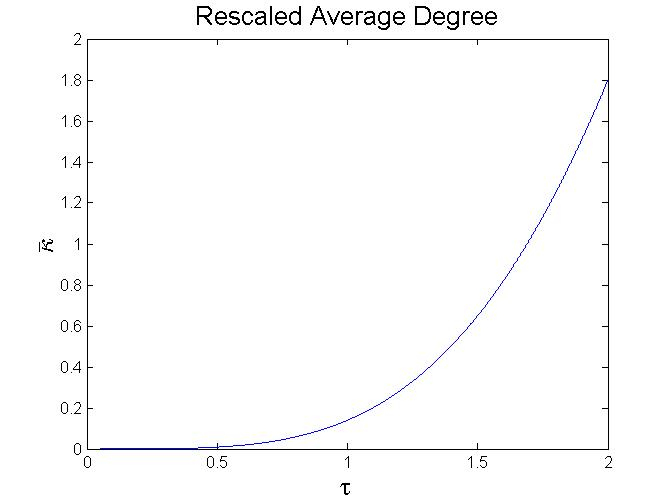
\includegraphics[width=10cm]{figures/Rescaled_Average_Degree.jpg}
\caption{Rescaled Average Degree of the Universe Causet}
\label{fig:kappa_tau}
\centering
\end{figure}

\paragraph{Method 2: Explicit Derivation}
An alternative approach has also been studied to verify the integrity of this method.
When the conformal time, scale factor, and expected average degree are rescaled in~\cite{ref:snc2012} it is not necessarily clear how the pseudoradius and scaling constant $\alpha$ could implicitly affect the results.
To show the above method is correct, the expected average in-degree is calculated directly using

\begin{equation}
\label{eq:avg_degree_uni}
\bar{k}_i\left(\eta^\prime|\eta\right) = \frac{4}{3}\pi\delta\int_{\eta^\prime}^\eta\!\left(\eta^{\prime\prime} - \eta^\prime\right)^3 R^4\left(\eta^{\prime\prime}\right)\,\mathrm d\eta^{\prime\prime}
\end{equation}

\noindent which can be recognized as (89) in~\cite{ref:snc2012}. \par
%%%%%%%%%%
The primary difficulty in evaluating this expression is that we must find an analytical expression for the scale factor in terms of the conformal time.
We know the scale factor in terms of cosmic (and therefore rescaled) time, and we know how to solve for a given conformal time from a given rescaled time (see~\eqref{eq:t_to_eta} and~\eqref{eq:scale_factor} for exact expressions) but we require an expression which has the form $R\left(\tau\left(\eta\right)\right)$ which involves inverting~\eqref{eq:t_to_eta}.
With a little bit of math and a single lookup table this is possible. \par
%%%%%%%%%%
First, we need a method for approximating \eqref{eq:t_to_eta}.
This can be accomplished using the Gauss Hypergeometric function and its associated transformations.
The integral can be rewritten in the following form (see Appendix~\ref{sec:alt_conformal} for a more complete derivation):

\begin{equation}
\begin{split}
\eta\left(\tau, a, \alpha\right) = \frac{2a}{3\alpha}\left(-1\right)^{5/6}&\left[\cosh\left(\frac{3}{2}\tau\right) {}_2F_1\left(\frac{1}{2},\frac{5}{6},\frac{3}{2};\cosh^2\left(\frac{3}{2}\tau\right)\right)\right. \\
& \quad - \left.\frac{\sqrt{\pi}\Gamma\left(1/6\right)}{2\Gamma\left(2/3\right)}\right]
\end{split}
\end{equation}

\noindent However, to use the power series approximation for the hypergeometric term we must apply the transformation described by~\eqref{eq:2F1transform}.
This allows the expression to be simplified to

\begin{equation}
\begin{split}
\label{eq:conformal_final}
\eta\left(\tau, a, \alpha\right) = \frac{a}{9\alpha\Gamma\left(2/3\right)}&\left[3\Gamma\left(-1/3\right)\sech^{2/3}\left(\frac{3}{2}\tau\right) {}_2F_1\left(\frac{1}{3},\frac{5}{6},\frac{4}{3};\sech^2\left(\frac{3}{2}\tau\right)\right)\right. \\
& \quad + \left.\frac{4\sqrt{3}\pi^{3/2}}{\Gamma\left(5/6\right)}\right]
\end{split}
\end{equation}

\noindent and so by using a lookup table we can return a value of $\tau$ for any given $\eta$.
To be clear, this expression is useful primarily because it allows us to calculate the conformal time by using a power series approximation, which is far faster than the previous method which uses numerical integration. \par
%%%%%%%%%%
As an intermediate check, let us confirm this alternative expression for conformal time is correct by comparing it to (91) in~\cite{ref:snc2012}.
We should find the expression~\eqref{eq:conformal_final} is equal to

\begin{equation}
\frac{2a}{\alpha}\sinh^{1/3}\left(\frac{3}{2}\tau\right) {}_2F_1\left(\frac{1}{6},\frac{1}{2},\frac{7}{6},-\sinh^2\left(\frac{3}{2}\tau\right)\right)
\end{equation}

\noindent Note that the rescaled scale factor has been substituted in this expression so both are a function of rescaled time.
When these functions are evaluated over a range of values (with the help of Mathematica) it is clear \textbf{the two expressions are equal}.
We define the functions

\begin{align}
f\left(\tau\right) &= \sech^{2/3}\left(\frac{3}{2}\tau\right) {}_2F_1\left(\frac{1}{3},\frac{5}{6},\frac{4}{3};\sech^2\left(\frac{3}{2}\tau\right)\right) \\
g\left(\eta, a, \alpha\right) &= \frac{1}{3\Gamma\left(-1/3\right)}\left(\frac{9\Gamma\left(2/3\right)\alpha}{a}\eta - \frac{4\sqrt{3}\pi^{3/2}}{\Gamma\left(5/6\right)}\right)
\end{align}

\noindent and we can find the scale factor as a function of conformal time by using $R\left(\eta\right) = R\left(f^{-1}\left(g\left(\eta, a, \alpha\right)\right)\right)$.
This is possible because the function $f\left(\tau\right)$ is a monotonically decreasing function, shown in Fig.~\ref{fig:f_tau_tau}.
The values generated in the table correspond directly to the domain shown in the figure.
Note that the function is finite at $\tau = 0$.
Then, the average in- and out-degree should be

\begin{figure}
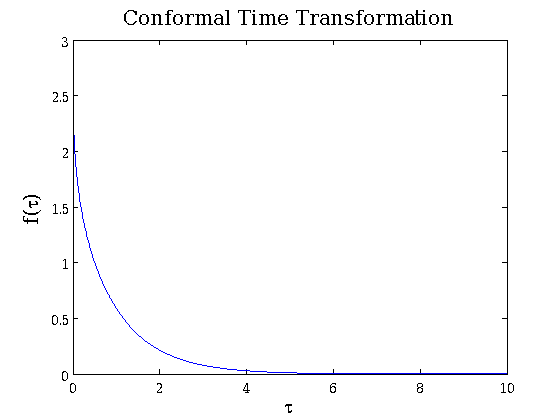
\includegraphics[width=10cm]{figures/ctuc.png}
\caption{Conformal Time Lookup Table}
\label{fig:f_tau_tau}
\centering
\end{figure}

\begin{align}
\bar{k}_i\left(\eta^\prime|\eta_0\right) &= \frac{4\pi\delta\alpha^4}{3}\int_{\eta^\prime}^{\eta_0}\!\left(\eta^{\prime\prime}-\eta^\prime\right)^3\sinh^{8/3}\left(\frac{3}{2}f^{-1}\left(g\left(\eta^{\prime\prime}, a, \alpha\right)\right)\right)\,\mathrm d\eta^{\prime\prime} \\
\bar{k}_o\left(\eta^\prime|\eta_0\right) &= \frac{4\pi\delta\alpha^4}{3}\int_0^{\eta^\prime}\!\left(\eta^\prime-\eta^{\prime\prime}\right)^3\sinh^{8/3}\left(\frac{3}{2}f^{-1}\left(g\left(\eta^{\prime\prime}, a, \alpha\right)\right)\right)\,\mathrm d\eta^{\prime\prime}
\end{align}

\noindent The average degree is found by adding these two expressions and integrating over the density function

\begin{equation}
\rho\left(\eta^\prime|\eta\right) &= \frac{R^4\left(\eta^\prime\right)}{\mathcal{N}_2\left(\eta\right)} \\
\mathcal{N}_2\left(\eta\right) &= \int_0^\eta\!R^4\left(\eta^\prime\right)\,\mathrm d\eta^\prime
\end{equation}

\noindent to obtain the desired result:

\begin{equation}
\label{eq:alt_avg_deg}
\bar{k}\left(\eta_0,a,\alpha\right) &= \frac{4\pi\delta\alpha^8}{3\mathcal{N}_2}\int_0^{\eta_0}\int_0^{\eta_0}\,\abs{\eta^\prime - \eta^{\prime\prime}}^3 r^4\left(\eta^\prime\right)r^4\left(\eta^{\prime\prime}\right)\,\mathrm d\eta^\prime\,\mathrm d\eta^{\prime\prime}
\end{equation}

\noindent The final expression~\eqref{eq:alt_avg_deg} is evaluated by numerically evaluating a 2-D and a 1-D integral (the latter for normalization) and by utilizing the lookup table in the 2-D integration.
Results are shown for the two methods below over a range of parameters.
For these tests, the number of nodes is held constant at $N = 10240$ and the maximum rescaled time is held constant at $\tau_0 = 1.8$.
First, the pseudoradius is held constant at $a = 1$ while $\alpha$ is varied and then subsequently $\alpha$ is held constant at $\alpha = 2$ while the pseudoradius $a$ is varied.
The two methods agree closely for all of these constraints, and any small discrepancies are likely due to errors associated with numerical integration.

\begin{center}
\begin{tabular}{|c||c|c|c||c|c|c|}
  \hline
  & \multicolumn{3}{|c||}{$a = 1$} & \multicolumn{3}{|c|}{$\alpha = 2$} \\ \hline
  & $\alpha = 0.8$ & $\alpha = 1.1$ & $\alpha = 1.4$ & $a = 0.8$ & $a = 1.1$ & $a = 1.4$ \\ \hline
  $\bar{k}_K$ & 72.300 & 27.812 & 13.490 & 2.369 & 6.159 & 12.697 \\ \hline
  $\bar{k}_W$ & 71.974 & 27.843 & 13.538 & 2.381 & 6.167 & 12.652 \\
  \hline
\end{tabular}
\end{center}

%%%%%%%%%%
\subsubsection{The Maximum Time}
%%%%%%%%%%
One of the most basic constrained parameters is the maximum conformal and rescaled time of the graph.
It serves to define the temporal boundary on the volume of the spacetime patch.  
Hence, if nodes are uniformly sprinkled at constant density then this maximum time may be calculated from the total number of nodes.
In a 1+1 patch of spacetime without matter it is easy to derive the relation from the definition of the differential volume element

\begin{equation}
\begin{split}
\mathrm{d}V &= \left(a\sec\eta\right)^{\mathrm{d}+1}\,\mathrm{d}\eta\,\mathrm{d}\Phi_d \\
   &= a^2\sec^2\eta\,\mathrm{d}\eta\,\mathrm{d}\theta_3
\end{split}
\end{equation}

\noindent Integration yields the volume

\begin{equation}
\begin{split}
V &= a^2\int_0^{\eta_0}\!\mathrm{d}\eta\int_0^{2\pi}\!\mathrm{d}\theta_3\,\sec^2\eta \\
  &= 2\pi a^2\int_0^{\eta_0}\!\sec^2\eta\,\mathrm{d}\eta \\
  &= 2\pi a^2\tan\eta_0
\end{split}
\end{equation}

\noindent and with some algebra this simplifies to the following relation

\begin{equation}
\label{eq:finalN1}
N_{\mathrm{1+1}} = 2\pi\delta a^2\tan\eta_0
\end{equation}

\noindent The same procedure may be applied to derive a similar relation in a 3+1 patch of spacetime without matter

\begin{equation}
\mathrm{d}V = a^4\sec^4\eta\,\mathrm{d}\eta\,\sin^2\theta_1\,\sin\theta_2\,\mathrm{d}\theta_1\,\mathrm{d}\theta_2\,\mathrm{d}\theta_3
\end{equation}

\noindent Integrate the differential volume element to get the total volume

\begin{equation}
\begin{split}
V &= a^4\int_0^{\eta_0}\!\mathrm{d}\eta\int_0^{2\pi}\!\mathrm{d}\theta_3\int_0^\pi\!\mathrm{d}\theta_2\int_0^\pi\!\mathrm{d}\theta_1\,\sec^4\eta\,\sin^2\theta_1\,\sin\theta_2 \\
  &= 2\pi a^4\int_0^{\eta_0}\!\mathrm{d}\eta\int_0^\pi\!\mathrm{d}\theta_2\int_0^\pi\!\mathrm{d}\theta_1\,\sec^4\eta\,\sin^2\theta_1\,\sin\theta_2 \\
  &= 4\pi a^4\int_0^{\eta_0}\!\mathrm{d}\eta\int_0^\pi\!\mathrm{d}\theta_1\,\sec^4\eta\,\sin^2\theta_1 \\
  &= 2\pi^2 a^4\int_0^{\eta_0}\!\sec^4\eta\,\mathrm{d}\eta \\
  &= \frac{2}{3}\pi^2 a^4\,\left(2+\sec^2\eta_0\right)\,\tan\eta_0
\end{split}
\end{equation}

\noindent and multiply by the scaled density to get the number of nodes

\begin{equation}
\label{eq:finalN3}
N_{\mathrm{3+1}} = \frac{2}{3}\pi^2\delta a^4\,\left(2+\sec^2\eta_0\right)\,\tan\eta_0
\end{equation}

\noindent Recall in a 3+1 patch of spacetime with matter, the maximum rescaled time is an independent parameter (supposing we let $\bar{k}$ be a dependent parameter).
In this case, the function solves for the maximum conformal time from the maximum rescaled time.
The transformation is given by equations (52), (85), and (86) in~\cite{ref:snc2012}:

\begin{align}
\eta &= \int_0^t\!\frac{\mathrm dt^\prime}{R\left(t^\prime\right)} \label{eq:t_to_eta} \\
R\left(t\right) &= \alpha\sinh^{\frac{2}{3}}\left(\frac{3t}{2a}\right) \label{eq:scale_factor}
\end{align}

\noindent where~\eqref{eq:scale_factor} was derived earlier in~\eqref{eq:scale_factor_derivation}.
These combine to produce

\begin{equation}
\eta_0 = \frac{1}{\alpha}\int_0^{a\tau_0}\!\sinh^{-\frac{2}{3}}\left(\frac{3t^\prime}{2a}\right)\,\mathrm dt^\prime
\end{equation}

\noindent This is calculated numerically using 1-D QNG integration in the GNU Scientific Library.  It may also be approximated with a power series.  This technique is described in detail in the appendix. \par
%%%%%%%%%%
It is often desirable to hold the average degree approximately constant rather than the density of nodes or the pseudoradius.  
In the cases with no matter (i.e. pure energy) the maximum conformal time may be solved via a transcendental equation if the average degrees is specified as an independent parameter.
In a 1+1 spacetime patch the distribution of nodes in the temporal dimension is given by

\begin{equation}
\rho = \frac{\sec^2\eta}{\tan\eta_0}
\end{equation}

\noindent with the volume of the past light cone of the event at $\eta$ written as

\begin{equation}
V_p = 2a^2\ln\sec\eta
\end{equation}
\noindent With some algebra the expected volume becomes

\begin{equation}
\begin{split}
V_p &= 2a^2\int_0^{\eta_0}\!\frac{\sec^2\eta}{\tan\eta_0}\,\ln\,\sec\eta\,\mathrm{d}\eta \\
  &= \frac{2a^2}{\tan\eta_0}\,\lbrack\eta + \tan\eta\left(\ln\,\sec\eta - 1\right)\rbrack_0^{\eta_0} \\
  &= \frac{2a^2}{\tan\eta_0}\,\lbrack\eta_0 + \tan\eta_0\left(\ln\,\sec\eta_0 - 1\right)\rbrack \\
  &= 2a^2\left(\frac{\eta_0}{\tan\eta_0} + \ln\,\sec\eta_0 - 1\right)
\end{split}
\end{equation}

\noindent Similarly, the volume of the future light cone of the event at $\eta$ is

\begin{equation}
V_f = 2a^2\left(\left(\eta_0 - \eta\right)\,\tan\eta_0 + \ln\,\left(\frac{\sec\eta}{\sec\eta_0}\right)\right)
\end{equation}

\noindent and the expected volume of the future light cone becomes

\begin{equation}
\begin{split}
V_f &= 2a^2\int_0^{\eta_0} \! \frac{\sec^2\eta}{\tan\eta_0} \left[\left(\eta_0 - \eta\right)\,\tan\eta_0 + \ln\left(\frac{\sec\eta}{\sec\eta_0}\right) \right]\,\mathrm{d}\eta \\
  &= \frac{2a^2}{\tan\eta_0}\left[\eta_0\tan\eta_0\int_0^{\eta_0}\!\sec^2\eta\,\mathrm{d}\eta - \tan\eta_0 \int_0^{\eta_0}\!\eta\sec^2\eta\,\mathrm{d}\eta\right. \\ & \left.\,\,\,\,\, + \int_0^{\eta_0}\!\sec^2\eta\ln\sec\eta\,\mathrm{d}\eta - \ln\sec\eta_0\int_0^{\eta_0}\!\sec^2\eta\,\mathrm{d}\eta\right] \\
  &= \frac{2a^2}{\tan\eta_0}\left[\eta_0\tan^2\eta_0 - \eta_0\tan^2\eta_0 + \tan\eta_0\ln\sec\eta_0\right. \\ & \left.\,\,\,\,\, + \eta_0 + \tan\eta_0\left(\ln\sec\eta_0 - 1\right) - \tan\eta_0\ln\sec\eta_0\right] \\
  &= 2a^2\left(\frac{\eta_0}{\tan\eta_0} + \ln\sec\eta_0 - 1\right)
\end{split}
\end{equation}

\noindent We now see the two expected volumes are indeed equal

\begin{align}
V_p &= V_f \\
\bar{k} &= \delta\left( V_p + V_f \right)
\end{align}
\noindent and we arrive at the final result for a 1+1 patch:

\begin{equation}
\label{eq:finalk1}
\bar k = 4 \delta a^2 \left( \frac{\eta_0}{\tan\eta_0} + \ln\sec\eta_0 - 1 \right)
\end{equation}

\noindent By taking together the two equations~\eqref{eq:finalN1} and~\eqref{eq:finalk1} we find the maximum conformal time may be found by solving the transcendental equation

\begin{equation}
\label{eq:trans1}
\frac{\bar k}{N} = \frac{2}{\pi}\frac{\eta_0 / \tan\eta_0 + \ln\sec\eta_0 - 1}{\tan\eta_0}
\end{equation}

\noindent A similar strategy may applied to a 3+1 patch of spacetime with no matter.  The volume of the past light cone is given by the expression

\begin{align}
V_p\left(\eta\right) &= \int_0^\eta \! \mathrm d\eta^\prime \, \int_0^{\eta-\eta^\prime} \! \mathrm d\theta_1 \, \int_0^{2\pi}\!\mathrm d\theta_3\, \int_0^\pi\!\mathrm d\theta_2\, a^4\sec^4\eta^\prime\sin^2\theta_1\sin\theta_2 \\
  &= 2a^4\int_0^\eta\!\mathrm d\eta^\prime\, \int_0^{\eta-\eta^\prime}\!\mathrm d\theta_1\, \int_0^{2\pi}\!\mathrm d\theta_3\, \sec^4\eta^\prime\sin^2\theta_1 \\
  &= 4\pi a^4 \int_0^\eta\!\mathrm d\eta^\prime\,\int_0^{\eta-\eta^\prime}\!\mathrm d\theta_1\, \sec^4\eta^\prime\sin^2\theta_1 \\
  &\qquad\begin{aligned}
    \int_0^{\eta-\eta^\prime}\!\sin^2\theta_1\,\mathrm d\theta_1 = \frac{1}{2}\left[\eta-\eta^\prime\right.&\left.+\sin\eta\cos\eta\left(1-2\cos^2\eta^\prime\right)\right. \\
    &\left.-\sin\eta^\prime\cos\eta^\prime\left(1-2\cos^2\eta\right)\right]
  \end{aligned} \\
  &\begin{aligned}
    = 2\pi a^4\int_0^\eta\!\mathrm d\eta^\prime\,\sec^4\eta^\prime\left[\eta-\eta^\prime\right.&\left.+\left(1-2\cos^2\eta^\prime\right)\sin\eta\cos\eta\right. \\
    &\left.-\sin\eta^\prime\cos\eta^\prime\left(1-2\cos^2\eta\right)\right]
  \end{aligned} \\
  &\qquad\int_0^\eta\!\eta\sec^4\eta^\prime\,\mathrm d\eta^\prime = \frac{\eta}{3}\tan\eta\left(2+\sec^2\eta\right) \\
  &\qquad\begin{aligned}
    \int_0^\eta\!\eta^\prime\sec^4\eta^\prime\,\mathrm d\eta^\prime = \frac{1}{3}\left[\right.&\left.-\ln\sec^2\eta-\frac{1}{2}\sec^2\eta + \frac{1}{2}\right. \\
    &\left.+2\eta\tan\eta+\eta\sec^2\eta\tan\eta\right]
  \end{aligned} \\
  &\qquad\int_0^\eta\!\left(1-2\cos^2\eta^\prime\right)\sec^4\eta^\prime\sin\eta\cos\eta\,\mathrm d\eta^\prime = -\frac{4}{3}\sin^2\eta+\frac{1}{3}\tan^2\eta \\
  &\qquad\int_0^\eta\!\sin\eta^\prime\cos\eta^\prime\sec^4\eta^\prime\left(1-2\cos^2\eta\right)\,\mathrm d\eta^\prime = \frac{1}{2}\left(2\cos^2\eta+\sec^2\eta-3\right) \\
  &= \frac{2\pi a^4}{3}\left[\ln\sec^2\eta-\sec^2\eta+4-4\sin^2\eta+tan^2\eta-3\cos^2\eta\right] \\
  &= \frac{2\pi a^4}{3}\left[\ln\sec^2\eta-\sec^2\eta+\tan^2\eta+\cos^2\eta\right]
\end{align}

\noindent The temporal distribution of nodes is described by

\begin{equation}
\label{eq:rhoeta3}
\rho = \frac{3\sec^4\eta}{\left(2+\sec^2\eta_0\right)\tan\eta_0}
\end{equation}

\noindent and so we obtain the average out-degrees

\begin{align}
\bar{k_o} &= \delta\int_0^{\eta_0}\!\rho\left(\eta\right)V_p\left(\eta\right)\,\mathrm d\eta \\
  &= \frac{2\pi\delta a^4}{\left(2+\sec^2\eta_0\right)\tan\eta_0}\int_0^{\eta_0}\!\left[\sec^4\eta\ln\sec^2\eta - \sec^6\eta + \tan^2\eta\sec^4\eta+\sec^2\eta\right]\,\mathrm d\eta \\
  &\qquad\begin{aligned}
    \int_0^{\eta_0}\!\sec^4\eta\ln\sec^2\eta\,\mathrm d\eta = &\frac{4}{3}\eta_0 - \frac{10}{9}\tan\eta_0 + \frac{4}{3}\tan\eta_0\ln\sec\eta_0 \\
    &-\frac{2}{9}\sec^2\eta_0\tan\eta_0 + \frac{2}{3}\sec^2\eta_0\tan\eta_0\ln\sec\eta_0
  \end{aligned} \\
  &\qquad\int_0^{\eta_0}\!\sec^6\eta\,\mathrm d\eta = \frac{8}{15}\tan\eta_0 + \frac{4}{15}\tan\eta_0\sec^2\eta_0 + \frac{1}{5}\tan\eta_0\sec^4\eta_0 \\
  &\qquad\int_0^{\eta_0}\!\tan^2\eta\sec^4\eta\,\mathrm d\eta = -\frac{2}{15}\tan\eta_0 - \frac{1}{15}\tan\eta_0\sec^2\eta_0 + \frac{1}{5}\tan\eta_0\sec^4\eta_0 \\
  &\qquad\int_0^{\eta_0}\!\sec^2\eta\,\mathrm d\eta = \tan\eta_0 \\
  &=\frac{2\pi\delta a^4}{2+\sec^2\eta_0}\left[\frac{4}{3}\frac{\eta_0}{\tan\eta_0} - \frac{7}{9} + \frac{4}{3}\ln\sec\eta_0 - \frac{5}{9}\sec^2\eta_0 + \frac{2}{3}\sec^2\eta_0\ln\sec\eta_0\right]
\end{align}

\noindent Once again recognizing the two expected volumes are equal saves some work

\begin{equation}
\bar{k} = 2\bar{k_o}
\end{equation}

\noindent and we arrive at the final result:

\begin{equation}
\label{eq:finalk3}
\bar k = \frac{4}{9}\frac{\pi\delta a^4}{2+\sec^2\eta_0}\left[12\left(\frac{\eta_0}{\tan\eta_0}+\ln\sec\eta_0\right)+\left(6\ln\sec\eta_0-5\right)\sec^2\eta_0-7\right]
\end{equation}

\noindent Again, the resulting transcendental equation is this time obtained by combining~\eqref{eq:finalN3} and~\eqref{eq:finalk3} to get

\begin{equation}
\label{eq:trans3}
\frac{\bar k}{N} = \frac{2}{3\pi}\frac{12\left(\eta_0/\tan\eta_0 + \ln\sec\eta_0\right) + \left(6\ln\sec\eta_0 - 5\right)\sec^2\eta_0 - 7}{\left(2+\sec^2\eta_0\right)^2\tan\eta_0}
\end{equation}

\noindent In a pure-energy de Sitter universe we have the relation between rescaled and conformal times given by 

\begin{equation}
\sec\eta = \cosh\frac{t}{a}
\end{equation}

\noindent so at this point it is easy to obtain the rescaled time for pure-energy graphs.
%%%%%%%%%%
\subsubsection{Memory}
The next step requires allocating the data structures used to define a graph.  
A graph is defined by the coordinates of its events as well as its adjacency list.  
The list of coordinates takes 4 x 4 x N bytes at floating point precision.
The number of in- and out-degrees associated with each node is also saved - these use 4 x N bytes each.
Since edges are sparse it is more economical to use an adjacency list rather than an adjacency matrix.
Both the past and future edges (associated with in- and out-degrees respectively) are saved so that any given node can be analyzed independent from the rest of the graph.  
Each takes 4 x (N x $\bar k$ / 2) bytes.  
Since the actual average number of edges for a graph may be above the average of the ensemble, a buffer of 20\% is added.
Additionally, two indices pointing to locations in the adjacency lists are associated with each node to indicate where to start for a given node (the sparse pointers).
These take 4 x N bytes each.
Finally, a fraction of nodes indicated by the \textit{core\_edge\_ratio} parameter is allocated for an adjacency matrix so that subroutines looking for edges among the hubs (earliest events) do not suffer from long lookup times in the adjacency lists.  
This by default is set to 1\%.
Memory is allocated and deallocated in other locations in the code as well, such as in low-level GPU functions, but the memory segments described here represent the minimal requirement to store a single graph.
Moreover, all of these variables remain active and accessible throughout the duration of the simulation and are not freed until the very end.
%%%%%%%%%%
\subsubsection{Generating Nodes}
%%%%%%%%%%
Generating the spacetime coordinates of the nodes is the next task.  
In \textit{d}+1 dimensions we draw \textit{d} spatial coordinates from the surface of a unit \textit{d}-sphere.  
In a 1+1 de Sitter graph this consists of uniformly drawing an angle $\theta_3$ between 0 and $2\pi$.  
In a 3+1 spacetime two more angles $\theta_1$ and $\theta_2$ are drawn from the distributions $\left(2/\pi\right)\sin^2\theta_1$ and $\left(1/2\right)\sin\theta_2$ respectively between 0 and $\pi$. \par
%%%%%%%%%%
On the other hand, generating the temporal coordinates is different for each topology.
When there is no matter, conformal times are drawn between 0 and $\eta_0$:

\begin{align}
\rho_{1+1}\left(\eta|\eta_0\right) &= \frac{\sec^2\eta}{\tan\eta_0} \\
\rho_{3+1}\left(\eta|\eta_0\right) &= \frac{3\sec^4\eta}{\left(2+\sec^2\eta_0\right)\tan\eta_0}
\end{align}

\noindent When dust matter is present rescaled times are drawn between 0 and $\tau_0$ from the distribution

\begin{equation}
\label{eq:rhotau3}
\rho_{3+1}\left(\tau|\tau_0\right) = \frac{6\sinh^2\left(\frac{3}{2}\tau\right)}{\sinh\left(3\tau_0\right) - 3\tau_0}
\end{equation}

\noindent This distribution is shown in Figure~\ref{fig:tau_cdf} for the indicated parameter.
For each node, both its conformal and rescaled time are stored in memory to avoid redundant calculations in the measurement stages.
This requires only 4 x N extra bytes of memory so the tradeoff is worthwhile.

\begin{figure}
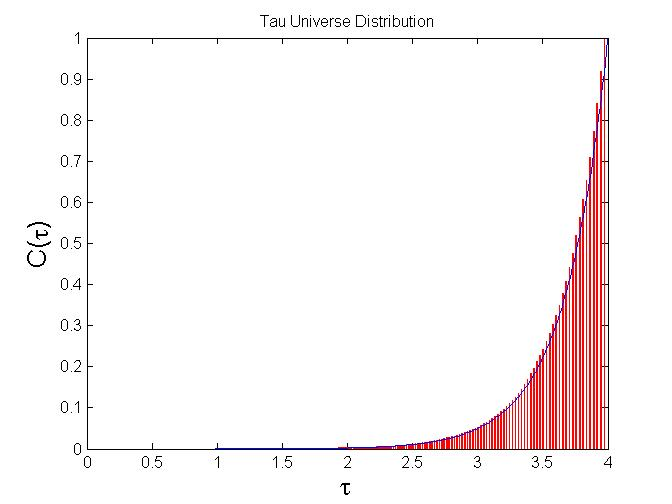
\includegraphics[width=10cm]{figures/tau_dist.jpg}
\caption{Cumulative distribution function of rescaled times for $\tau$ = 4.  The blue curve represents the theoretical distribution.}
\label{fig:tau_cdf}
\centering
\end{figure}

%%%%%%%%%%
\subsubsection{Linking Nodes with the CPU}
%%%%%%%%%%
Two events are said to be connected if there is a causal relation between them.  
Mathematically, this means if the Lorentzian inner product $\langle \vec x - \vec y, \vec x - \vec y\rangle$ is negative then the events are time-like separated and the two nodes located at coordinates $x$ and $y$ are connected.  
If the inner product is positive the events are space-like separated and the two nodes remain disconnected.
Define a four vector $\vec x = \left(\eta, \theta_1, \theta_2, \theta_3\right)$ with the metric signature $\left(-1,+1,+1,+1\right)$.
The temporal difference is easy:

\begin{equation}
\Delta\eta = \abs{x_0 - y_0}
\end{equation}

\noindent where $\eta$ is the conformal time of an event.  
For a single spatial dimension, the spatial distance is defined as the shortest arc length between two points on a $d$-sphere.  
It always lies between 0 and $\pi$.
In one spatial dimension this is given by

\begin{equation}
\Delta\theta = \pi - \abs{\pi - \abs{x_3 - y_3}}
\end{equation}

\noindent and in three spatial dimensions it is found using the spherical law of cosines to be

\begin{equation}
\begin{split}
\cos\left(\Delta\theta\right) = &\cos x_1\cos y_1 + \\
  &\sin x_1\cos x_2\sin y_1\sin y_2 + \\
  &\sin x_1\sin x_2\cos x_3\sin y_1\sin y_2\cos y_3 + \\
  &\sin x_1\sin x_2\sin x_3\sin y_1\sin y_2\sin y_3
\end{split}
\end{equation}

\noindent Now if the spacetime interval defined by the metric signature as $ds^2 = -d\eta^2 + d\theta^2$ is negative, two events are connected, so for every pair of nodes generated they will be linked if $\Delta\theta < \Delta\eta$.  \par
%%%%%%%%%%
When a pair is recognized as begin causally connected, several things then happen in the algorithm.
If both of the nodes are represented in the adjacency matrix, its binary value at this spot (and the one representing the reciprocal link) is set to true.
After, the earlier node's out-degree counter is incremented and the later node's in-degree counter is incremented.
Then, the earlier node's index is added to the list of past edges and the later node's index is added to the list of future edges.
Each time a node gets it's first neighbor added to an edge list, the index of the new edge's location in the edge list is added to the respective sparse pointer list.
If a node never has any past/future/any neighbors the sparse pointer values are set to -1.
Nodes must be temporally ordered for this to work correctly. \par
%%%%%%%%%%
After this operation, some non-zero percent of the nodes generated will be completely isolated and the rest will form connected components, often creating a giant connected component.
This makes it easy to identify the resulting averge degree and number of nodes (i.e. size of giant component).  
It is important to have these two values be very close to their target values so that there are not large statistical fluctuations between different graphs in a network.
Small fluctuations mean there is a large degree of control over the graphs produced by any given parameters, so the measured values have higher precision.
The number of nodes of degree two or higher is also calculated since it's a useful statistical quantity.
%%%%%%%%%%
\subsubsection{Linking Nodes with the GPU}
%%%%%%%%%%

\begin{figure}
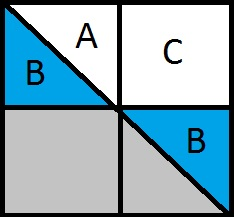
\includegraphics[width=5cm]{figures/Matrix_Map.jpg}
\caption{The lower right triangle B is mapped to the upper left quadrant, creating two square matrices which can be handled much more efficiently by the GPU.}
\label{fig:matrix_map}
\centering
\end{figure}

By performing the node-linking step in parallel, the network generation can occur tens or hundreds of times faster.
The pairwise comparison may be viewed as non-zero elements of an upper triangular matrix (Fig.~\ref{fig:matrix_map}).
In greater detail, splitting this matrix into four quadrants yields a triangular portion in both the upper-left and lower-right quadrants and a full square matrix in the upper-right quadrant.
By mapping the lower-right quadrant's values to the lower triangle in the upper-left quadrant, we are left with two densely packed square matrices in the upper half of the original matrix, each of width $width$. \par
%%%%%%%%%%
If $N(N-1)/4$ threads are launched, each thread can compare two pairs of nodes - one in the upper left quadrant and one in the upper-right quadrant of the original matrix.
For the purposes of this algorithm, threads indexed in the upper triangle of the upper-left quadrant is designated with the \textit{a} label, the lower triangle of the same quadrant with the \textit{b} label, and the upper right-quadrant with the \textit{c} label.  
Hence, each thread addresses an \textit{a} or \textit{b} pair as well as a \textit{c} pair.  
The method for determining the four nodes assigned to a given thread is shown below:

\begin{lstlisting}
	unsigned int tid = threadIdx.x;
	unsigned int i = blockIdx.y;
	unsigned int j = blockDim.x * blockIdx.x + threadIdx.x;
	int do_map = i >= j;

	unsigned int i_ab = i + do_map * (((width - i) << 1) - 1);
	unsigned int j_ab = j + do_map * ((width - j) << 1);

	unsigned int i_c = i;
	unsigned int j_c = j + width;
\end{lstlisting}

\noindent Several of these parameters are related to the block and grid size send to the kernel.  
Here, there are 128 threads per block, so \textit{tid} can range from 0 to 127.  
It is a 1-D thread block, so \textit{blockDim.y} = 1 and \textit{threadIdx.y} = 0 for all threads. \par
%%%%%%%%%%
Since the thread block is linear, one of the nodes read by each thread will be identical among all threads in the block.
To minimize reads to global GPU memory, this value is read to \textit{shared} memory by a single thread, after which the other 127 threads in the block will read it from the shared memory cache.
This is demonstrated by the following code snippet:

\begin{lstlisting}
	__shared__ float4 shr_node0_c;
	if (!tid)
		shr_node0_c = nodes[i_c];
	__syncthreads();

	float4 node0_c = shr_node0_c;
	float4 node0_ab = do_map ? nodes[i_ab] : node0_c;
\end{lstlisting}

\noindent In this example, the threads must be synchronized so that no reads from shared memory occur before the value is written from global memory.  
Further, it is possible elements in the \textit{a} triangular matrix will use the same value from shared memory, as demonstrated by the last line. \par
%%%%%%%%%%
While connections will in general be sparse, there will typically be multiple edges found in a given thread block.  
To avoid serializing writes to global memory with the \textit{atomicAdd} function, it is best to perform a reduction operation in the shared memory cache.  
The basic math involved in calculating \textit{dx} and \textit{dt} has been omitted.

\begin{lstlisting}
	__shared__ int n_a[BLOCK_SIZE];
	__shared__ int n_b[BLOCK_SIZE];
	__shared__ int n_c[BLOCK_SIZE];
	int edge_ab = dx_ab < dt_ab;
	int edge_c = dx_c < dt_c;

	n_a[tid] = edge_ab * !do_map;
	n_b[tid] = edge_ab * do_map;
	n_c[tid] = edge_c;
	__syncthreads();

	int stride;
	for (stride = 1; stride < BLOCK_SIZE; stride <<= 1) {
		if (!(tid % (stride << 1)) {
			n_a[tid] += n_a[tid+stride];
			n_b[tid] += n_b[tid+stride];
			n_c[tid] += n_c[tid+stride];
		}
		__syncthreads();
	}
\end{lstlisting}

\noindent This results in the total number of out-degrees for each region being stored in the inital spot of the respective arrays.  
This allows a single atomic operation to be performed per thread block for the out-degrees.  
The in-degrees must still be written by each thread, but this is guaranteed to avoid serialization (to the greatest extent possible) by the nature of how the thread block is designed.

\begin{lstlisting}
	if (edge_ab)
		atomicAdd(&k_in[j_ab], 1);
	if (edge_c)
		atomicAdd(&k_in[j_c], 1);

	if (!tid) {
		if (n_a[0])
			atomicAdd(&k_out[i], n_a[0]);
		if (n_b[0])
			atomicAdd(&k_out[i_ab], n_b[0]);
		if (n_c[0])
			atomicAdd(&k_out[i_c], n_c[0]);
	}
\end{lstlisting}

\noindent Finally, the edges are written to a single edge list of 64-bit integers by storing each pair $(i,j)$ in global memory, in a segment reserved via a final atomic operation on a global index.  
It is written in this manner because it is both easy to sort and it allows for contiguous writes to a single global memory segment.

\begin{lstlisting}
	int idx = 0;
	if (edge_ab | edge_c)
		idx = atomicAdd(g_idx, edge_ab + edge_c);
	if (edge_ab)
		edges[idx++] = ((uint64_t)i_ab) << 32 | ((uint64_t)j_ab);
	if (edge_c)
		edges[idx] = ((uint64_t)i_c) << 32 | ((uint64_t)j_c);
\end{lstlisting}
%%%%%%%%%%

\section{Measurements}
%description/purpose
%analytical/theoretical
%algorithmic design
%parameters tested
%results (plots)
%validations
%any conclusions
%%%%%%%%%%
\subsection{The Minimum Time}
%%%%%%%%%%
It is important to study the average minimum time generated in simulation for a given set of parameters because these nodes are the hubs.
Though their creation is a rare process, they have a profound effect on many properties of the resulting graph.
They affect the average degree, the connectivity, and the degree distributions.
Because the addition or deletion of a single hub can greatly affect the structure of a graph, choosing too few nodes in simulation can undersample them and therefore skew results.
Here we show a few examples of the minimum time for a few sets of parameters.

%%%%%%%%%%
\subsection{Average Degrees}
%%%%%%%%%%
We expect the expected average degrees of a network to be a Poissonian distribution about the mean value $\langle\bar{k}\rangle$.  
Because points are scattered via a Poisson process, the fluctuations from the average degrees will be Poissonian in their form.
We see the simulation results in Fig.~\ref{fig:avg_deg_uni} for several sets of parameters.

\begin{figure}
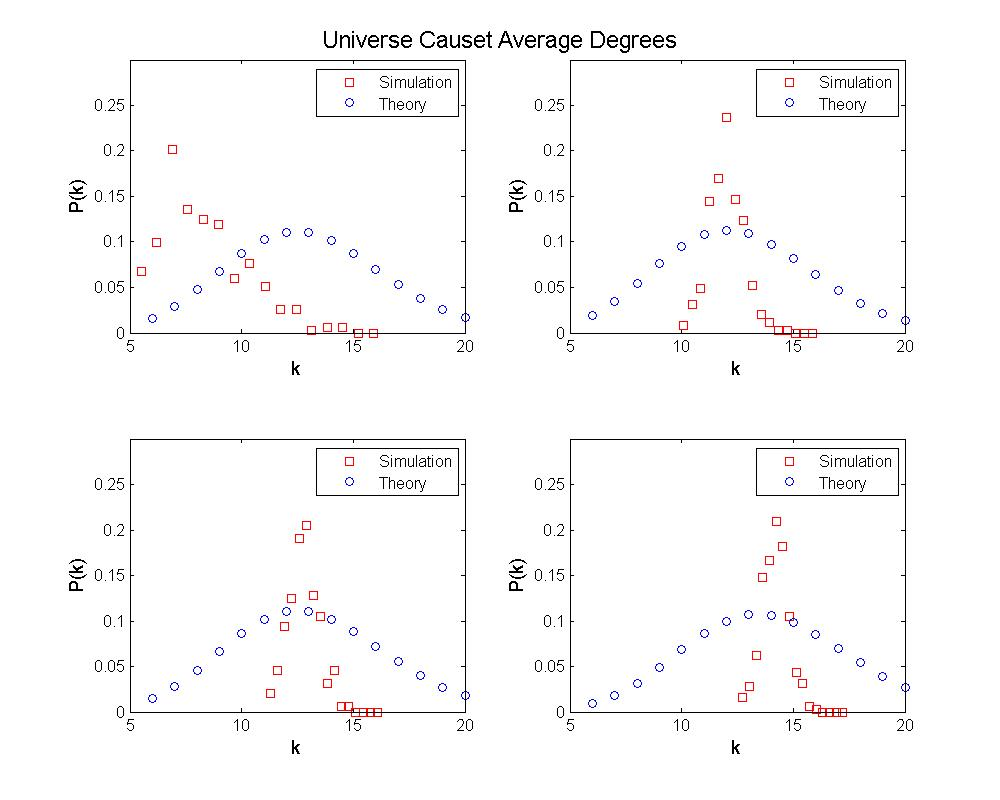
\includegraphics[width=18cm]{figures/avg_degrees.jpg}
\caption{Each of these graphs shows the average degree distribution for $a = 1$.  The small simulations are done using $N = 10240$ nodes over approximately 400 graphs and the large simulations are done using $N = 131072$ nodes over 100 graphs.  In the upper left graph, $\delta = 1$ and $\tau_0 = 4.0$.  In the upper right graph, $\delta = 10$ and $\tau_0 = 1.8$.  In the lower left graph, $\delta = 20$ and $\tau_0 = 1.5$.  In the lower right graph, $\delta = 150$ and $\tau_0 = 0.9$.}
\label{fig:avg_deg_uni}
\centering
\end{figure}

%%%%%%%%%%
\subsection{Connectivity}
%%%%%%%%%%
It is of interest to understand how the connectivity of the network changes as a function of the independent variables of the model.
By studying 100 graphs we obtained statistics about the number of isolated nodes, the number of connected components, and the size of the giant component.
%%%%%%%%%%
\subsubsection{Isolated Nodes}
%%%%%%%%%%
The number of isolated nodes may be solve analytically for a 1+1 spacetime with no matter.  For a poisson point process the probability function has the form

\begin{equation}
P(x) = \frac{\left(\delta V\right)^x}{x!}e^{-\delta V}
\end{equation}

\noindent The probability a node is isolated at conformal time $\eta$ is given by this expression, where $x=0$ is the number of nodes in the sum of the light cone volumes $V=V_p\left(\eta\right)+V_f\left(\eta\right)$.  
Manipulating this expression yields

\begin{equation}
\begin{split}
P\left(0\right) &= e^{-2\delta a^2\left[\left(\eta_0-\eta\right)\tan\eta_0 + \ln\sec^2\eta - \ln\sec\eta_0\right]} \\
  &= e^{-2\delta a^2\left[\eta_0\tan\eta_0 - \ln\sec\eta_0\right]}e^{-2\delta a^2\left[\ln\sec^2\eta - \eta\tan\eta_0\right]} \\
  &=\xi e^{-2\delta a^2\left[\ln\sec^2\eta-\eta\tan\eta_0\right]}
\end{split}
\end{equation}

\noindent Then, the expected number of isolated nodes is given by

\begin{equation}
\begin{split}
\langle N\left(0\right)\rangle &= N\int_0^{\eta_0}\!\rho\left(\eta\right)P\left(0\right)\,\mathrm d\eta \\
  &= \frac{N\xi}{\tan\eta_0}\int_0^{\eta_0}\!\sec^2\eta e^{-2\delta a^2\left[\ln\sec^2\eta - \eta\tan\eta_0\right]}\,\mathrm d\eta \\
  &\qquad e^{-2\delta a^2\ln\sec^2\eta} = \left(\cos\eta\right)^{4\delta a^2} \\
  &= \frac{N\xi}{\tan\eta_0}\int_0^{\eta_0}\left(\cos\eta\right)^{4\delta a^2 - 2} e^{\left(2\delta a^2 \tan\eta_0\right)\eta}\,\mathrm d\eta
\end{split}
\end{equation}

\noindent It is possible to simplify this further by recognizing the following identity:

\begin{equation}
\begin{split}
\int_0^a\!\cos^bxe^{cx}\,\mathrm dx = &\frac{\left(1+e^{2ia}\right)e^{ac}\cos^ba}{c-ib} {}_2F_1\left(1,\frac{b}{2}+1-i\frac{c}{2};1-\frac{b}{2}-i\frac{c}{2};-e^{2ia}\right) \\
& - \frac{2}{c-ib} {}_2F_1\left(1,\frac{b}{2}+1-i\frac{c}{2};1-\frac{b}{2}-i\frac{c}{2};-1\right)
\end{split}
\end{equation}

\noindent so in the present case we find

\begin{equation}
\begin{split}
\int_0^{\eta_0}\!\left(\cos\eta\right)^{4\delta a^2 - 2}&e^{2\delta a^2\eta\tan\eta_0}\,\mathrm d\eta = \left[\frac{\left(1+e^{2i\eta_0}\right)e^{2\delta a^2\eta_0\tan\eta_0}\left(\cos\eta_0\right)^{4\delta a^2 - 2}}{2\delta a^2\tan\eta_0 - i\left(4\delta a^2 - 2\right)}\right. \\
&\left.\times{}_2F_1\left(1,2\delta a^2 - i\delta a^2\tan\eta_0;2-2\delta a^2 - i\delta a^2\tan\eta_0;-e^{2i\eta_0}\right)\right] \\
& - \left[\frac{1}{\delta a^2\tan\eta_0 - i\left(2\delta a^2 - 1\right)}\right. \\
&\left.\times{}_2F_1\left(1,2\delta a^2-i\delta a^2\tan\eta_0;2-2\delta a^2-i\delta a^2\tan\eta_0;-1\right)\right]
\end{split}
\end{equation}

\noindent therefore we find the number of isolated nodes can be written as

\begin{equation}
\begin{split}
\bar{N}_0 &\sim N\frac{e^{-2\delta a^2\eta_0\tan\eta_0}\left(\cos\eta_0\right)^{-2\delta a^2}}{\tan\eta_0}\frac{\left(1+e^{2i\eta_0}\right)e^{2\delta a^2\eta_0}\left(\cos\eta_0\right)^{4\delta a^2-2}}{2\delta a^2\tan\eta_0 - i\left(4\delta a^2 - 2\right)} \\
& \quad\times {}_2F_1\left(1,2\delta a^2 - i\delta a^2\tan\eta_0;2-2\delta a^2 - i\delta a^2\tan\eta_0;-e^{2i\eta_0}\right) \\
&\sim N\frac{\left(1+e^{2i\eta_0}\right)\left(\cos\eta_0\right)^{2\delta a^2 - 2}}{2\delta a^2\left(\tan\eta_0\right)^2} {}_2F_1\left(1,2\delta a^2-i\delta a^2\tan\eta_0;2-2\delta-i\delta a^2\tan\eta_0;-e^{2i\eta_0}\right) \\
&\sim N\frac{\left(1+e^{2i\eta_0}\right)\left(\cos\eta_0\right)^{2\delta a^2}}{2\delta a^2} {}_2F_1\left(1,2\delta a^2-i\delta a^2\tan\eta_0;2-2\delta-i\delta a^2\tan\eta_0;-e^{2i\eta_0}\right)
\end{split}
\end{equation}

\noindent This can be reduced by implementing the Pfaff transformation:

\begin{equation}
{}_2F_1\left(a,b;c;z\right) = \left(1-z\right)^{-a} {}_2F_1\left(a,c-b;c;\frac{z}{z-1}\right)
\end{equation}

\noindent we find the relation

\begin{equation}
\begin{split}
\bar{N}_0 \sim &N\frac{\left(1+e^{2i\eta_0}\right)\left(\cos\eta_0\right)^{2\delta a^2}}{2\delta a^2}\left(1+e^{2i\eta_0}\right)^{-1} \\
&\quad \times {}_2F_1\left(1,2-4\delta a^2;2-2\delta a^2-i\delta a^2\tan\eta_0;\frac{e^{2i\eta_0}}{1+e^{2i\eta_0}}\right)
\end{split}
\end{equation}

\noindent and by using the approximations (as $\eta_0\to\frac{\pi}{2}$)

\begin{equation}
e^{2i\eta_0}\to -1;\quad 1+e^{2i\eta_0}\to 2i\left(\frac{\pi}{2} - \eta_0\right);\quad \tan\eta_0\to\frac{1}{\frac{\pi}{2}-\eta_0}
\end{equation}

we arrive at the equation

\begin{equation}
\begin{split}
\bar{N}_0 &\sim N\frac{\left(\cos\eta_0\right)^{2\delta a^2}}{2\delta a^2} {}_2F_1\left(1,2-4\delta a^2;\frac{-i\delta a^2}{\frac{\pi}{2}-\eta_0};\frac{-1}{2i\left(\frac{\pi}{2}-\eta_0\right)}\right) \\
&\sim N\frac{\left(\cos\eta_0\right)^{2\delta a^2}}{2\delta a^2} {}_2F_1\left(1,2-4\delta a^2;-i\delta a^2\tan\eta_0;\frac{i}{2}\tan\eta_0\right)
\end{split}
\end{equation}

Since the average number of isolated nodes is known to be a real number, it makes sense to continue to reduce this expression to eliminate the complex quantities.  
To do this, we need to apply four new relations:

\begin{enumerate}
  \item For $a - b\notin \mathbb{Z}$ and $x\notin\left(0, 1\right)$,
  \begin{equation}
    \label{eq:2F1transform}
    \begin{split}
    {}_2F_1\left(a,b;c;x\right) =& \frac{\Gamma\left(b-a\right)\Gamma\left(c\right)}{\Gamma\left(b\right)\Gamma\left(c-b\right)}\left(-x\right)^{-a} {}_2F_1\left(a,a-c+1;a-b+1;\frac{1}{x}\right) + \\
    & \frac{\Gamma\left(a-b\right)\Gamma\left(c\right)}{\Gamma\left(a\right)\Gamma\left(c-b\right)}\left(-x\right)^{-b} {}_2F_1\left(b,b-c+1;-a+b+1;\frac{1}{x}\right)
    \end{split}
  \end{equation}

  \item The Kummer hypergeometric function is
  \begin{equation}
  {}_1F_1\left(a;c;bd\right) = \lim_{x\to\infty} {}_2F_1\left(a,bx;c;\frac{d}{x}\right)
  \end{equation}

  \item
  \begin{equation}
  \lim_{x\to\infty}\frac{\Gamma\left(x\right)}{\Gamma\left(x-a\right)} = x^a
  \end{equation}

  \item
  \begin{equation}
  \label{eq:1F1_limit}
  {}_1F_1\left(1;a;b\right) = \left(a-1\right)e^{b}b^{1-a}\left(\Gamma\left(a-1\right)-\Gamma\left(a-1,b\right)\right)
  \end{equation}
\end{enumerate}

\noindent By using the definitions $\alpha\equiv 2-4\delta a^2$, $\beta\equiv -i\delta a^2$, $\gamma\equiv\frac{i}{2}$, and $x\equiv\tan\eta_0$ and the relations

\begin{equation}
\begin{split}
{}_2F_1\left(1,\alpha;\beta x;\gamma x\right) &= \frac{\Gamma\left(\alpha-1\right)\Gamma\left(\beta x\right)}{\Gamma\left(\alpha\right)\Gamma\left(\beta x-1\right)}\left(-\gamma x\right)^{-1} {}_2F_1\left(1,2-\beta x;2-\alpha;\frac{1}{\gamma x}\right) \\
&\quad + \frac{\Gamma\left(1-\alpha\right)\Gamma\left(\beta x\right)}{\Gamma\left(1\right)\Gamma\left(\beta x-\alpha\right)}\left(-\gamma x\right)^{-\alpha} {}_2F_1\left(\alpha,\alpha+1-\beta x;\alpha;\frac{1}{\gamma x}\right) \\
&\rightarrow \frac{\beta x-1}{\left(\alpha-1\right)\left(-\gamma x\right)} {}_1F_1\left(1;2-\alpha;-\frac{\beta}{\gamma}\right) \\
&\quad + \frac{\Gamma\left(1-\alpha\right)\left(\beta x\right)^\alpha}{\left(-\gamma x\right)^\alpha} {}_1F_1\left(\alpha;\alpha;-\frac{\beta}{\gamma}\right)
\end{split}
\end{equation}
\noindent as well as the limit with~\eqref{eq:1F1_limit}, we obtain

\begin{equation}
\lim_{x\to\infty} {}_2F_1\left(1,\alpha;\beta x;\gamma x\right) = e^{-\beta/\gamma}\left(-\frac{\beta}{\gamma}\right)^\alpha\Gamma\left(1-\alpha,-\frac{\beta}{\gamma}\right)
\end{equation}

\noindent and finally arrive at the result

\begin{equation}
\bar{N}_0 \sim N\left(e\cos\eta_0\right)^{2\delta a^2}\left(2\delta a^2\right)^{1-4\delta a^2}\Gamma\left(4\delta a^2-1,2\delta a^2\right)
\end{equation}

\noindent For a 3+1 spacetime it does not appear to be possible to obtain a closed-form analogue of this solution.  

%1+1 for N = 24586, k = 5.53
%3+1 for N = 25441, k = 5.29

\par For a 3+1 universe with matter, we have found the following results for the number of isolated nodes:

\begin{figure}
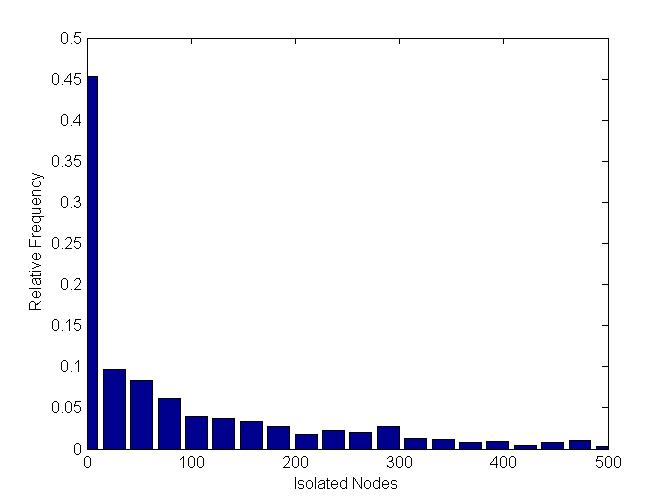
\includegraphics[width=10cm]{figures/Isolated_Nodes.jpg}
\caption{The distribution of isolated nodes taken over a sample of 1000 graphs.  These graphs were constrained by the parameters $N = 10240$, $\tau_0 = 4$, $a = 1$, and $\delta = 1$.}
\label{fig:iso_nodes_uni}
\centering
\end{figure}

\subsubsection{Number of Connected Components}
In this project we are interested in networks above the percolation threshold, so in all cases the average degree has been manipulated to meet this condition.  
The number of connected components was calculated by implementing a breadth first search algorithm, assigning each node an identification number associated with a component.
Beginning at the earliest node, the algorithm works by assigning each past and future neighbor the same component ID as the current node, so the algorithm acts recursively.  Once each pass is completed, the second earliest node is checked to see if it has been assigned a component ID.  If it has not, the recursive process is repeated.  This is done for every node until every single one has a component ID.

%1+1 for N = 24586, k = 5.53
%3+1 for N = 25441, k = 5.29

\begin{figure}
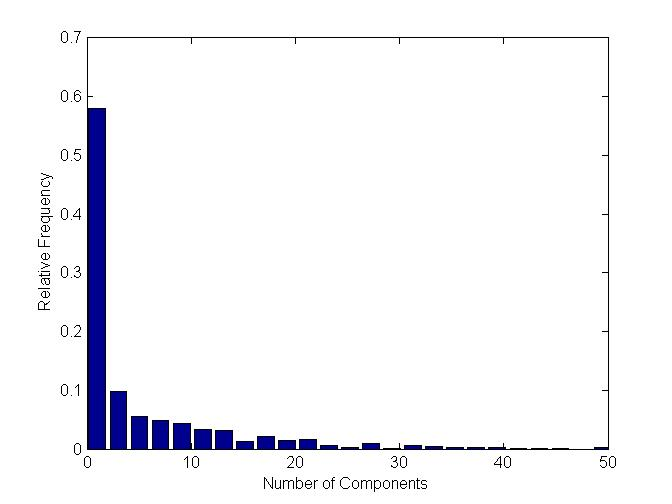
\includegraphics[width=10cm]{figures/Number_Components.jpg}
\caption{The distribution of connected components taken over a sample of 1000 graphs.  These were constrained by the parameters $N = 10240$, $\tau_0 = 4$, $a = 1$, and $\delta = 1$.}
\label{fig:num_comp_uni}
\centering
\end{figure}

\subsubsection{Size of Giant Component}
The size of the giant component is similar to the number of isolated nodes except when the system is below the percolation threshold.  
Since all components except for the giant component are ignored it was useful to identify any possible deviations in statistical behavior through this extra quantity.
When the breadth first search algorithm is used, if it is performed first on the earliest node (the largest hub) then any nodes with the same component ID as the hub are recognized as part of the giant component.
Therefore by counting the number of nodes which have matching IDs it is easy to find the size of the giant component.

%1+1 for N = 24586, k = 5.53
%3+1 for N = 25441, k = 5.29

\begin{figure}
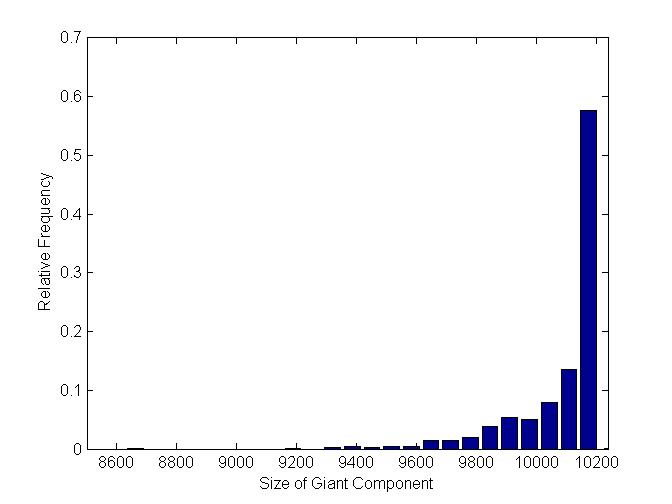
\includegraphics[width=10cm]{figures/Giant_Component.jpg}
\caption{The size of the giant component in a sample of 1000 graphs.  These were constrained by the parameters $N = 10240$, $\tau_0 = 4$, $a = 1$, and $\delta = 1$. \XXX{wc}{kz}{It would be interesting to see the plot of the expected relative size of the giant component $\langle\mathcal{G}\rangle/N$ as a function of $\bar{k}$ and $a$, } \XXX{kz}{wc}{I'll add this.}}
\label{fig:size_gcc_uni}
\centering
\end{figure}

\subsection{Degree Distribution}
Numerical evaluation of the degree distributions for a universe with matter can be done using these equations from~\cite{ref:snc2012}:

\begin{align}
\bar{k}_i\left(\eta^\prime|\eta\right) &= \delta\frac{\pi}{K}\int_{\eta^\prime}^\eta\!\left\{2\left(\eta^{\prime\prime} - \eta^{\prime}\right) - \frac{1}{\sqrt{K}}\sin\left[2\sqrt{K}\left(\eta^{\prime\prime} - \eta^{\prime}\right)\right]\right\}R^4\left(\eta^{\prime\prime}\right)\, \mathrm d\eta^{\prime\prime} \\
\bar{k}_o\left(\eta^\prime|\eta\right) &= \delta\frac{\pi}{K}\int_0^{\eta^\prime}\!\left\{2\left(\eta^{\prime\prime} - \eta^{\prime}\right) - \frac{1}{\sqrt{K}}\sin\left[2\sqrt{K}\left(\eta^{\prime\prime} - \eta^{\prime}\right)\right]\right\}R^4\left(\eta^{\prime\prime}\right)\, \mathrm d\eta^{\prime\prime} \\
p\left(k|\eta^\prime,\eta\right) &= \frac{1}{k\!}\left[\bar{k} \left(\eta^\prime|\eta\right)\right]^k e^{-\bar{k} \left(\eta^\prime|\eta\right)} \\
\rho\left(\eta^\prime|\eta\right) &= \frac{R^4\left(\eta^\prime\right)}{\mathcal N \left(\eta\right)} \\
P\left(k,\eta\right) &= \int_0^\eta\! p\left(k|\eta^\prime,\eta\right)\rho\left(\eta^\prime|\eta\right)\,\mathrm d\eta^\prime
\end{align}

\subsubsection{In-Degree Distribution}
The in-degrees describe connections coming into a given node from an earlier node.
See Fig.~\ref{fig:in_deg_uni} for a comparison of simulation results to theory.

\begin{figure}
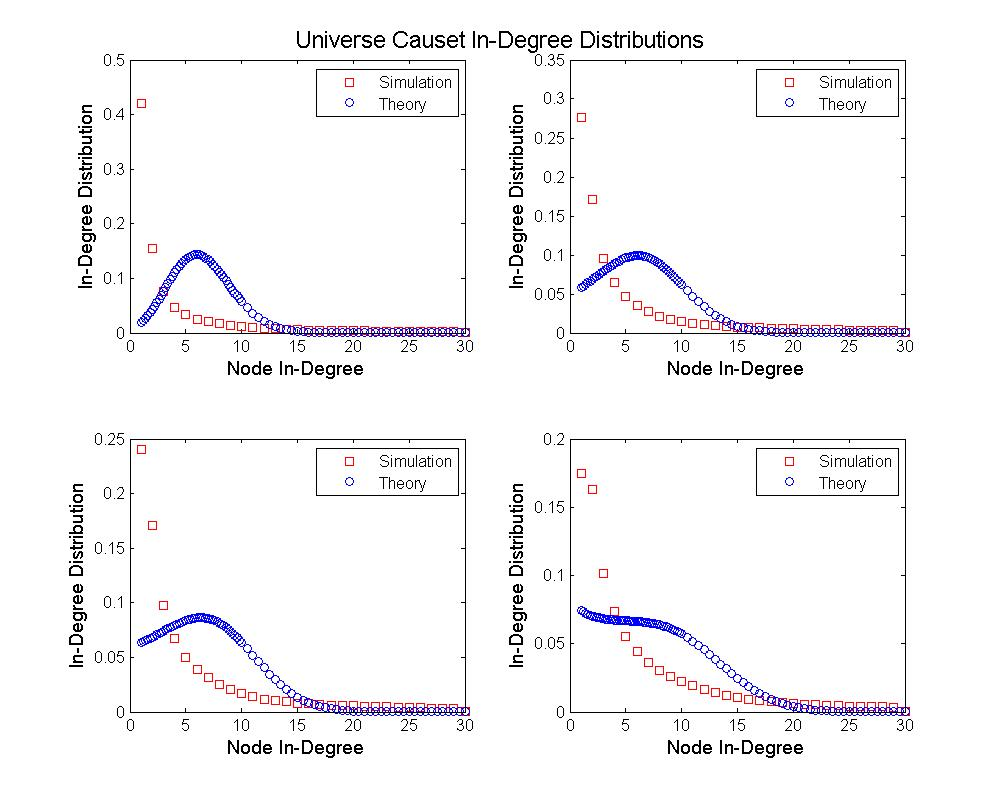
\includegraphics[width=18cm]{figures/in_degrees.jpg}
\caption{Each of these graphs shows the in-degree distribution for $a = 1$.  The small simulations are done using $N = 10240$ nodes over approximately 400 graphs and the large simulations are done using $N = 131072$ nodes over 100 graphs.  In the upper left graph, $\delta = 1$ and $\tau_0 = 4.0$.  In the upper right graph, $\delta = 10$ and $\tau_0 = 1.8$.  In the lower left graph, $\delta = 20$ and $\tau_0 = 1.5$.  In the lower right graph, $\delta = 150$ and $\tau_0 = 0.9$.}
\label{fig:in_deg_uni}
\centering
\end{figure}

\subsubsection{Out-Degree Distribution}
Likewise, the out-degrees describe connections exiting a given node toward a node at a later time.  The same parameters have been tested to produce the plots shown in Fig.~\ref{fig:out_deg_uni}.

\begin{figure}
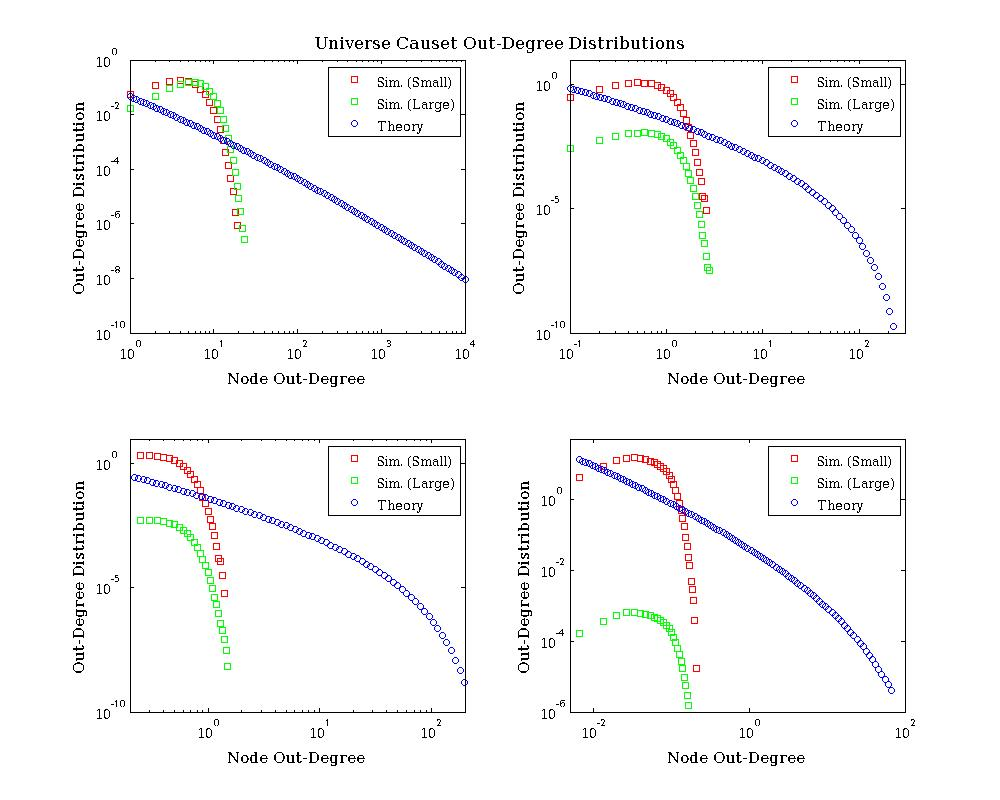
\includegraphics[width=18cm]{figures/out_degrees.jpg}
\caption{Each of these graphs shows the \textbf{rescaled} out-degree distribution for $a = 1$.  The small simulations are done using $N = 10240$ nodes over approximately 400 graphs and the large simulations are done using $N = 131072$ nodes over 100 graphs.  In the upper left graph, $\delta = 1$ and $\tau_0 = 4.0$.  In the upper right graph, $\delta = 10$ and $\tau_0 = 1.8$.  In the lower left graph, $\delta = 20$ and $\tau_0 = 1.5$.  In the lower right graph, $\delta = 150$ and $\tau_0 = 0.9$.}
\label{fig:out_deg_uni}
\centering
\end{figure}

\begin{comment}

\subsection{Clustering}
\subsubsection{Average Clustering}
\subsubsection{Clustering Distribution}

\end{comment}

\subsection{Navigability in the Universe}
\subsubsection{Geodesic Distances in the Universe}
Measuring geodesic distances in an FLRW universe with a positive dark energy density and dust matter is currently an unsolved problem.  
We hypothesize that we may embed the 3+1 manifold isometrically in a higher spatial dimension so distances may be calculated using a 4+1 Lorentzian metric.  
This is not a problem for a simple de Sitter manifold, but the alterations to the topology resulting from the inclusion of matter may render this an incorrect approach.  
Here we propose a mathematical framework to justify the extension of the embedding technique to the new manifold, as well as several validation tests which may be performed in the causal set simulation. \par
%%%%%%%%%%
We begin by considering a flat five-dimensional Minkowski space $\mathbb{M}^{4+1}$

\begin{equation}
ds^2 = -dz_0^2 + dz_1^2 + dz_2^2 + dz_3^2 + dz_4^2,
\end{equation}

\noindent and the de Sitter manifold that is embedded in $\mathbb{M}^{4+1}$, $d\mathbb{S}^{3+1}\subset\mathbb{M}^{4+1}$

\begin{equation}
-z_0^2 + z_1^2 + z_2^2 + z_3^2 + z_4^2 = a^2, \quad a = \sqrt{3/\Lambda}
\end{equation}

\noindent $d\mathbb{S}^{3+1}$ can be covered by the coordinates $\left(t,\theta_1,\theta_2,\theta_3\right)$.  Let us rotate the system such that all the angular coordinates of a node are zero.  
Then we have

\begin{equation}
\begin{cases}
z_0 &= a\sinh\frac{t}{a} \\
z_1 &= a\cosh\frac{t}{a} \\
z_2 &= z_3 = z_4 = 0
\end{cases}
\end{equation}

\noindent Now we want to find a function $z_1 = f\left(z_0\right)$ such that 

\begin{equation}
\label{eq:length}
\begin{cases}
&z_1 = R\left(t\right) = a\cosh\frac{t}{a} \\
&L\left[\left(x,f\left(x\right)\right), x\in\left[0,z_0\right]\right] = t
\end{cases}
\end{equation}

\noindent where L is the length of the curve along the de Sitter manifold in the temporal direction.  In the Minkowski metric,

\begin{equation}
L = \int_0^{z_0}\!\sqrt{\abs{f^\prime\left(x\right)^2 - 1}}\,\mathrm dx
\end{equation}

Therefore, using~\eqref{eq:length} we have

\begin{equation}
\label{eq:embedded_z0}
f\left(z_0\right) = R\left(\int_0^{z_0}\!\sqrt{\abs{f^\prime\left(x\right)^2-1}}\,\mathrm dx\right)
\end{equation}

For $d\mathbb{S}^{3+1}$, we know that $R\left(t\right) = a\cosh\frac{t}{a}$ and $f\left(z_0\right) = \sqrt{z_0^2+a^2}$.  As a test, let us check that~\eqref{eq:embedded_z0} is satisfied for this special case.

\begin{equation}
\begin{split}
\int_0^{z_0}\!\sqrt{\abs{f^\prime\left(x\right)^2-1}}\,\mathrm dx &= \int_0^{z_0}\!\sqrt{\abs{\frac{x^2}{x^2+a^2}-1}}\,\mathrm dx \\
&= \int_0^{z_0}\!\frac{a}{\sqrt{x^2+a^2}}\,\mathrm dx \\
&= a\int_0^{z_0}\!\frac{\mathrm d\frac{x}{a}}{\sqrt{\left(\frac{x}{a}\right)^2+1}} \\
&= a\int_0^{z_0/a}\!\frac{\mathrm dy}{\sqrt{y^2+1}} \\
&= a\sinh^{-1}\frac{z_0}{a}
\end{split}
\end{equation}

\begin{equation}
\begin{split}
f\left(z_0\right) &= a\cosh\left(\sinh^{-1}\frac{z_0}{a}\right) \\
&= a\sqrt{\frac{z_0^2}{a^2}+1} \\
&= \sqrt{z_0^2+a^2}
\end{split}
\end{equation}

\noindent Since the scale factor $R\left(t\right)$ is monotonic, we can invert $R\left(t\right)$ and obtain the transcendental differential equation

\begin{equation}
\frac{f^\prime\left(z_0\right)}{R^\prime\left(R^{-1}\left(f\left(z_0\right)\right)\right)} = \sqrt{\abs{1 - f^\prime\left(z_0\right)^2}}
\end{equation}

\noindent For a $\Lambda$CDM spacetime we obtain from this

\begin{align}
R\left(t\right) &= \alpha\sinh^\frac{2}{3}\left(\frac{3t}{2a}\right) \\
R^\prime\left(t\right) &= \frac{\alpha}{a}\frac{\cosh\left(\frac{3t}{2a}\right)}{\sinh^{1/3}\left(\frac{3t}{2a}\right)} \\
R^{-1}\left(t\right) &= \frac{2a}{3}\sinh^{-1}\left(\frac{t}{\alpha}\right)^{3/2} \\
R^\prime\left(R^{-1}\left(t\right)\right) &= \frac{\alpha}{a}\frac{\sqrt{1+\left(\frac{t}{\alpha}\right)^3}}{\sqrt{\frac{t}{\alpha}}}
\end{align}

\noindent so we get the result

\begin{equation}
\frac{f^\prime\left(z_0\right)}{\sqrt{\abs{1-f^\prime\left(z_0\right)^2}}} = \frac{\alpha^{3/2}}{a}\frac{\sqrt{1+\left(\frac{f\left(z_0\right)}{\alpha}\right)^2}}{\sqrt{f\left(z_0\right)}}
\end{equation}

Now, we would like to obtain an analogue of this equation for the function $z_0 = f\left(z_1\right)$.  We begin the derivation as before:

\begin{align}
z_1 &= R\left(\int_0^{z_1}\!\sqrt{\abs{1-f^\prime\left(x\right)^2}}\,\mathrm dx\right) \\
R^{-1}\left(z_1\right) &= \int_0^{z_1}\!\sqrt{\abs{1-f^\prime\left(x\right)^2}}\,\mathrm dx \\
\frac{\mathrm d}{\mathrm dz_1}R^{-1}\left(z_1\right) &= \sqrt{\abs{1-f^\prime\left(z_1\right)^2}} \\
\abs{1-f^\prime\left(z_1\right)^2} &= \left(\frac{\mathrm d}{\mathrm dz_1}R^{-1}\left(z_1\right)\right)^2 \\
f^\prime\left(z_1\right) &= \sqrt{1\pm\left(\frac{\mathrm d}{\mathrm dz_1}R^{-1}\left(z_1\right)\right)^2}
\end{align}

\noindent and we find the resulting general expression to be

\begin{equation}
f\left(z_1\right) = \int_0^{z_1}\!\sqrt{1\pm\left(\frac{\mathrm d}{\mathrm dx}R^{-1}\left(x\right)\right)^2}\,\mathrm dx
\end{equation}

\noindent When the scale factor for the $\Lambda$CDM spacetime is inserted into this expression we arrive at

\begin{equation}
f\left(z_1\right) = z_0 = \int_0^{z_1}\!\sqrt{1+\frac{a^2x\alpha^2}{\alpha^3+x^3}}\,\mathrm dx
\end{equation}

\begin{figure}
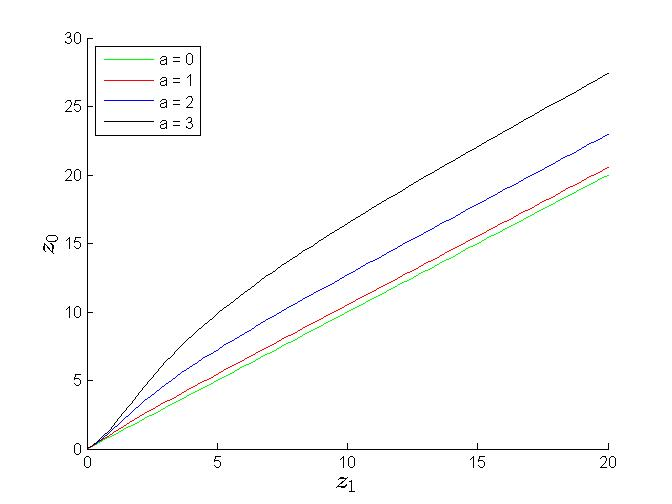
\includegraphics[width=10cm]{figures/Embedding.jpg}
\caption{Embedding function $z_0 = f\left(z_1\right)$ for the $\Lambda$CDM spacetime.}
\label{fig:embedding}
\centering
\end{figure}

\noindent where we have taken the positive sign in the $\pm$ to represent the physical situation.  A plot of this equation is shown in Fig.~\ref{fig:embedding} for several choices of parameters. \par
%%%%%%%%%%
The inner product between two vectors is always invariant under Lorentz transformations, so the two vectors may be rotated such that each of their spatial coordinates is zero.  
The scalar product of the two 5-D vectors in terms of the transformed coordinates is described by

\begin{align}
z^\prime_1 &= R\left(t\right) \\
z^\prime_0 &= \int_0^{z^\prime_1} \! \sqrt{1 + \frac{a^2x\alpha^2}{\alpha^3 + x^3}} \, \mathrm{d}x \\
\langle \vec{z}^\prime_a, \vec{z}^\prime_b \rangle &= -\left(z^\prime_0\right)_a \left(z^\prime_0\right)_b + \left(z^\prime_1\right)_a \left(z^\prime_1\right)_b
\end{align}

\noindent When rotated into the spatial planes by the angles $(\theta_1, \theta_2, \theta_3)$, we find the scalar product becomes 

\begin{align}
z_0 &= z^\prime_0 \\
z_1 &= z^\prime_1\cos\theta_1 \\
z_2 &= z^\prime_1\sin\theta_1\cos\theta_2 \\
z_3 &= z^\prime_1\sin\theta_1\sin\theta_2\cos\theta_3 \\
z_4 &= z^\prime_1\sin\theta_1\sin\theta_2\sin\theta_3 \\
\langle \vec{z}_a, \vec{z}_b \rangle &= -\left(z_0\right)_a\left(z_0\right)_b + \left(z_1\right)_a\left(z_1\right)_b + \left(z_2\right)_a\left(z_2\right)_b + \left(z_3\right)_a\left(z_3\right)_b + \left(z_4\right)_a\left(z_4\right)_b
\end{align}

The condition for calculating the distance is given by Definition 2.6 in~\cite{ref:asmus2009}.
If the vector $\vec{x}-\vec{y}$ is timelike, this means

\begin{equation}
\langle\vec x - \vec y,\vec x - \vec y\rangle < 0
\end{equation}

\begin{equation}
\vec{x}^2 - 2\vec{x}\cdot\vec{y} + \vec{y}^2 = 2\left(1-\vec{x}\cdot\vec{y}\right)
\end{equation}

\begin{equation}
\vec{x}\cdot\vec{y} > 1
\end{equation}

\noindent and then the distance is given by

\begin{equation}
d(\vec{x},\vec{y}) = \cosh^{-1}(\langle \vec{x}, \vec{y}\rangle)
\end{equation}

\noindent Geometrically this is the case where points lie on a great hyperbola.  
If the vector $\vec{x}-\vec{y}$ is lightlike (which does not occur for randomly distributed points) the distance is identically zero.  
If the inner product $\langle \vec{x},\vec{y}\rangle \leq -1$ then the distance is infinite since the plane defined by the two vectors intersects the de Sitter space is timelike, with the two points on disconnected components.  
If the vector $\vec{x}-\vec{y}$ is spacelike on the condition that $\langle \vec{x},\vec{y}\rangle \geq -1$ then

\begin{equation}
\vec{x}\cdot\vec{y} < 1
\end{equation}

\noindent and the distance is given by

\begin{equation}
d(\vec{x},\vec{y}) = \cos^{-1}(\langle \vec{x},\vec{y}\rangle)
\end{equation}

\noindent This represents the case where the points are connected by a great ellipse.

\XXX{wc}{kz}{After all explanations, can we write down a ready-to-use formula for computing distance between two nodes $n_a=(t_a,(\theta_1)_a,(\theta_2)_a,(\theta_3)_a)$  and $n_b=(t_b,(\theta_1)_b,(\theta_2)_b,(\theta_3)_b)$? (I still prefer to use $\phi, \theta,$ and $\chi$)} \XXX{kz}{wc}{I'll add this later.}

\subsubsection{Validation Test for Manifold Embedding}
One method of validating this approach is to calculate geodesic distances is to identify if time-like and space-like intervals in 3+1 de Sitter space are also classified as such in the embedded 4+1 manifold.  
If two nodes are connected when the network is constructed, the distance between the two points should be time-like.  
If not, it should be classified as space-like.  
There should be no light-like vectors because nodes are randomly distributed.
We can characterize the success of the embedding by defining the confusion matrix as follows:

\begin{equation}
C = \left( \begin{array}{cc}
\frac{S_4 \bigcap S_5}{S_4} & \frac{T_4 \bigcap S_5}{T_4} \\
\frac{S_4 \bigcap T_5}{S_4} & \frac{T_4 \bigcap T_5}{T_4} \end{array} \right)
\end{equation}

where S and T indicate space-like and time-like classifications respectively, and the subscripts indicate the number of dimensions used in the method with which they were classified.
For a universe with no matter (pure de Sitter) we expect this to be a unit matrix, and that is exactly what we find in simulation.
For the parameters $N = 10240$, $\tau_0 = 4$, $a = 1$, $\delta = 1$ and a random seed $-1406627360$ in the $\Lambda$CDM spacetime  we find the confusion matrix is

\begin{equation}
C = \left( \begin{array}{cc}
1.000 & 0.934 \\
0.000 & 0.066 \end{array} \right)
\end{equation}
\XXX{wc}{kz}{It seems that $T_5\approx0$ and $S_5\approx1$ and the network is essentially disconnected. What is $\bar{k}$ in this case, maybe it is too small? We need to see how entries of this matrix change with $\bar{k}$.} \XXX{kz}{wc}{This is something I will add.}

This indicates when the 4-D manifold is embedded in the fifth dimension using this set of constraints, $93.4\%$ of timelike pairs are misclassified as spacelike.
Figure X \XXX{wc}{kz}{Where is it?} \XXX{kz}{wc}{Not ready yet, I'll introduce it for a range of parameters.} indicates how misclassified distances vary as a function of $\Delta\theta$, $\Delta\eta$, and the pseudoradius $a$.

\begin{comment}

\begin{figure}[t]
\includegraphics[width=6in]{figures/TN_Dist.jpg}
\caption{Figure 3:  Distribution of True Negative Spatiotemporal Distances.}
\end{figure}

\end{comment}

\subsubsection{Limiting Cases}
Because we are using the pseudoradius as our variable parameter in the greedy routing experiment, it is useful to know the analytic expression for the asymptotic behavior of the matter and energy densities as $t_0$ (and therefore $a$) tends to zero and $\infty$.  We begin with the following definitions which were derived earlier:

\begin{align}
\rho_\Lambda &= \frac{3}{8\pi G}\frac{1}{a^2} \\
\rho_M &= \frac{3}{8\pi G}\left(a\sinh\frac{3\tau_0}{2}\right)^{-2} \\
t_0 &= \left(\frac{\bar k}{\delta\bar\kappa}\right)^{1/4}\tau_0
\end{align}

\noindent For the two densities we can drop the numerical coefficients since we are interested in asymptotic behavior only. \\
%%%%%%%%%%
\textbf{Statement:}
\begin{enumerate}
  \item
  \begin{align}
  \lim_{a\to 0} t_0 &= \infty \\
  \lim_{a\to\infty} t_0 &= \hat{t}_0\in\left(0,\infty\right)
  \end{align}

  \item
  \begin{align}
  \lim_{a\to 0} \rho_M &= 0 \\
  \lim_{a\to\infty} \rho_M &= \hat{\rho}_M\in\left(0,\infty\right)
  \end{align}
\end{enumerate}

\noindent To show this we need to find the asymptotic behavior of $\bar\kappa\left(\tau_0\right)$ as $\tau_0\to 0$ and $\tau_0\to\infty$. \\
%%%%%%%%%%
\textbf{Lemma:}

\begin{equation}
\bar{\kappa}\left(\tau_0\right) = 
\begin{cases}
\mathcal{O}\left(\tau_0^4\right) & \mathrm{as}\quad \tau_0\to 0 \\
\mathcal{O}\left(\tau_0\right) & \mathrm{as}\quad \tau_0\to\infty
\end{cases}
\end{equation}

\noindent Using this fact, we can find the dependence on the pseudoradius for the remaining two quantities.  For $t_0$ we find

\begin{equation}
t_0 = \left(\frac{\bar k}{\delta}\right)^{1/4}\frac{\tau_0}{\bar\kappa\left(\tau_0\right)^{1/4}}
\end{equation}

\begin{align}
\lim_{a\to 0} t_0 &= \lim_{\tau_0\to\infty} t_0 = \left(\frac{\bar k}{\delta}\right)^{1/4}\lim_{\tau_0\to\infty}\frac{\tau_0}{\mathcal{O}\left(\tau_0^{1/4}\right)} = \infty \\
\lim_{a\to\infty} t_0 &= \lim_{\tau_0\to 0} t_0 = \left(\frac{\bar k}{\delta}\right)^{1/4}\lim_{\tau_0\to\infty}\frac{\tau_0}{\mathcal{O}\left(\tau_0\right)} = \hat{t}_0
\end{align}

\noindent and for the density of matter we find

\begin{equation}
\begin{split}
\rho_M^\prime &= \frac{8\pi G}{3}\rho_M = \left(a\sinh\frac{3\tau_0}{2}\right)^{-2} = \left(\frac{\bar k}{\delta\bar\kappa\left(\tau_0\right)}\right)^{-1/2}\left(\sinh\frac{3\tau_0}{2}\right)^{-2} \\
&= \left(\frac{\delta}{\bar k}\right)^{1/2}\frac{\bar\kappa\left(\tau_0\right)^{1/2}}{\left(\sinh\frac{3\tau_0}{2}\right)^2}
\end{split}
\end{equation}

\begin{align}
\lim_{a\to 0}\rho_M^\prime &= \lim_{\tau_0\to\infty}\rho_M^\prime = \left(\frac{\delta}{\bar k}\right)^{1/2}\lim_{\tau_0\to\infty}\frac{\mathcal{O}\left(\tau_0\right)}{\mathcal{O}\left(e^{3\tau_0}\right)} = 0 \\
\lim_{a\to\infty}\rho_M^\prime &= \lim_{\tau_0\to 0}\rho_M^\prime = \left(\frac{\delta}{\bar k}\right)^{1/2}\lim_{\tau_0\to 0}\frac{\mathcal{O}\left(\tau_0^2\right)}{\mathcal{O}\left(\tau_0^2\right)} = \hat{\rho}_M^\prime
\end{align}

\XXX{wc}{kz}{Before we start experiments with greedy routing, we need to fix 2 things: 1) find for which values of parameters we can control $\bar{k}$ in simulated graphs, i.e. generate graphs with observed $\bar{k}$ close to the target one. First step is to fix $N$, $\delta$, and $a$, and to plot $\langle\bar{k}\rangle$ and $\langle\mathcal{G}\rangle/N$ as functions of $\bar{k}$; expectations can be estimated using, say 1000 realizations. 2) Fix the entries of confusion matrix. It must be close to the identity matrix, otherwise, our embedding and the corresponding computation of the distance do not make sense.}

\subsubsection{Greedy Routing Algorithm}
The following describes the greedy routing algorithm in terms of pseudocode
\begin{description}
  \item[INPUT]
\end{description}
\begin{itemize}[leftmargin=*]
  \item $N$ - List of 4-D node coordinates
  \item $N_{tar}$ - Target number of nodes in connected component
  \item $N_{sr}$ - Percent of node pairs to traverse (up to $\frac{N(N-1)}{2}$)
\end{itemize}
\begin{description}
  \item[START]
\end{description}
\begin{itemize}[leftmargin=*]
  \item [] \textbf{for each} pair $(i,j)$:
  \begin{itemize}[leftmargin=*]
    \item [] \textbf{If} $i == j$ \textbf{or} either node has no edges, \textbf{continue}
    \item [] \textbf{If} nodes in separate components, \textbf{continue}
    \item [] $loc = i$
    \item [] \textbf{while} $loc$ != $j$
    \begin{itemize}[leftmargin=*]
      \item [] $d_{min}$ = INF
      \item [] $next = loc$
      \item [] \textbf{for each} past neighbor pn:
      \begin{itemize}[leftmargin=*]
        \item [] \textbf{If} pn == j \textbf{then} loc = j; \textbf{break while}
        \item [] \textbf{If} distance($N_{pn}$, $N_j$) $< d_{min}$ \textbf{then} save new $d_{min}$ and $next$
      \end{itemize}
      \item [] \textbf{for each} future neighbor fn:
      \begin{itemize}[leftmargin=*]
        \item [] \textbf{If} fn == j \textbf{then} loc = j; \textbf{break while}
        \item [] \textbf{If} distance($N_{fn}$, $N_j$) $< d_{min}$ \textbf{then} save new $d_{min}$ and $next$
      \end{itemize}
      \item [] \textbf{If} $next$ has not been traversed \textbf{then} $loc = next$
      \item [] \textbf{Else break while} loop
    \end{itemize}
    \item [] \textbf{If} $loc == j$ \textbf{then} $R_s$ = $R_s$ + 1.0
    \item [] $N_{tr}$ = $N_{tr}$ + 1
  \end{itemize}
  \item [] $R_s$ = $R_s$ / $N_{tr}$
\end{itemize}
\begin{description}
  \item[OUTPUT]
\end{description}
\begin{itemize}[leftmargin=*]
  \item $R_s$ - Success ratio
  \item $N_{tr}$ - Number of traversed pairs
\end{itemize}

\begin{comment}

\subsubsection{Success Ratio}
Here we have tested several combinations of parameters:

%N = 10240, kbar = 12.90, delta = 1
%a = 0.9, 1.0, 1.1, 1.5, 2, 2.8, 3, 3.4, 4, 5

\section{Summary of Results}

\section{Latest Challenges}

\end{comment}

\appendix
\appendixpage
\addappheadtotoc

\section{Usage of the Causal Set Software}
%%%%%%%%%% 
The tasks in the program are broken into modular subroutines so that it can be used for diverse purposes.
Functions are divided in a hierarchical structure so that the main method only accesses high-level functions (described in \textit{Causets.cu}) with the entire \textit{Network} data structure.
In a similar fashion, these high-level functions strictly access low-level functions (in \textit{NetworkCreator.cu} and \textit{Measurements.cu}), and the low-level functions access mathematical (\textit{Operations.h}) and algorithmic (\textit{Subroutines.cu}) functions.
Debugging and other validation tests are located in the \textit{Validation.cu} file.
When the GPU is used, entire low-level functions are replaced (e.g. in \textit{NetworkCreator\_GPU.cu}) because the flow of information is entirely different. \par
%%%%%%%%%%
All tasks and parameters may be specified as command-line parameters - these may be queried using the \textbf{-h} or \textbf{--help} flags.
They are shown here alphabetically for the purposes of documentation.

\begin{description}
  \item[-A, --alpha] \tab Set unphysical free parameter used in the universe's causal set, described in (11) and (12) of~\cite{ref:snc2012}.
  \item[-a, --radius] \tab Set pseudoradius of spacetime.
  \item[-C, --clustering] \tab Calculate clustering coefficients and average clustering.
  \item[-c, --core] \tab Set fraction of nodes used in adjacency matrix.  
A hybrid method is used which minimizes both memory allocation and lookup times.
Typically this value is $\mathcal{O}(0.01)$ of all nodes.
  \item[-D, --delta] \tab Set node density.
  \item[-d, --dim] \tab Set number of spatial dimensions (1 or 3).
  \item[-E, --embedding] \tab Perform embedding validation test.  Space-like and time-like intervals are compared in the 3+1 and 4+1 universe's causal set.
  \item[-G, --components] \tab Calcualate size of the giant connected component and the number of smaller connected components.
  \item[-g, --graph] \tab Set graph ID.  
This is used to indicate a unique ID of an existing graph which the program reads and analyzes.
  \item[-h, --help] \tab Display this information.
  \item[-k, --degrees] \tab Set the average degrees of the graph.
  \item[-l, --lambda] \tab Set the cosmological constant.  
Related to the pseudoradius via the equation $\Lambda = \frac{3}{a^2}$.
  \item[-m, --manifold] \tab Indicate a [d]e Sitter or [h]yperbolic manifold.  Used to indicate the type of graph being read when the \textbf{-g} flag is used.
  \item[-n, --nodes] \tab Set the number of nodes to generate and attempt to link.
  \item[-o, --energy] \tab Set the dark energy density $\Omega_\Lambda$.
  \item[-r, --ratio] \tab Set the ratio of dark energy to matter $\frac{\Omega_\Lambda}{\Omega_M}$.
  \item[-S, --success] \tab Set the fraction of node pairs to use to study navigability and calculate the success ratio.
  \item[-s, --seed] \tab Set the random seed.
  \item[-T, --test] \tab Test parameters in the universe causal set to identify dependent constraints.
  \item[-t, --age] \tab Rescaled age $\tau_0$.
  \item[-u, --universe] \tab Indicate a causal set with dust matter (and Big Bang).
  \item[-v, --verbose] \tab Print verbose output when the program is run.
  \item[-y] \tab\tab Suppress user queries during the verbose output.
  \item[-z, --zeta] \tab Set the curvature of a hyperbolic manifold.
  \item[--autocorr] \tab Calculate autocorrelation of clustering coefficients.
  \item[--benchmark] \tab Benchmark subroutines and numerical algorithms.
  \item[--conflicts] \tab Show parameter conflicts for universe causal set.
  \item[--gpu] \tab Use GPU accelerated subroutines.
  \item[--print] \tab Print results to file in \textit{dat} folder.
\end{description}

\section{Alternative Expressions for the Conformal Time}
\label{sec:alt_conformal}
One of the most important numerical steps in the simulation involves identifying causally connected points, which necessarily uses the conformal time.  In the causal set representing the universe with matter, this requires solving

\begin{equation}
\eta\left(t\right) = \frac{1}{\alpha}\int_0^t\!\sinh^{-2/3}\left(\frac{3t^\prime}{2a}\right)\,\mathrm dt^\prime
\end{equation}

\noindent for every spacetime node.  An integral of this form can easily be expressed in terms of the Gauss Hypergeometric function by equating a binomial series expansion to the hypergeometric series.

\begin{equation}
\begin{split}
\int\!\sinh^nx\,\mathrm dx &= \int\!\sinh x\sinh^{n-1}x\,\mathrm dx \\
  &= \int\!\sinh x\left(\cosh^2x-1\right)^{\left(n-1\right)/2}\,\mathrm dx \\
  &= \left(-1\right)^{\left(1-n\right)/2}\int\!\sinh x\left(1-\cosh^2x\right)^{\left(n-1\right)/2}\,\mathrm dx \\
  &= \left(-1\right)^{\left(1-n\right)/2}\cosh x{}_2F_1\left(\frac{1}{2},\frac{1-n}{2};\frac{3}{2};\cosh^2x\right)
\end{split}
\end{equation}

\noindent In the present case, we have $n=-2/3$, which yields the following intermediate result

\begin{equation}
\eta\left(t\right) = \frac{2a}{3\alpha}\left(-1\right)^{5/6}\left[\cosh\left(\frac{3t}{2a}\right) {}_2F_1\left(\frac{1}{2},\frac{5}{6};\frac{3}{2};\cosh^2\left(\frac{3t}{2a}\right)\right) - \frac{\sqrt{\pi}\Gamma\left(1/6\right)}{2\Gamma\left(2/3\right)}\right]
\end{equation}

\noindent We can easily approximate the Hypergeometric function here by a power series, but only if the magnitude of its kernel function is less than one.  Since we know $\cosh^2x$ is always greater than one, we can implement the transformation~\eqref{eq:2F1transform} to get (after some algebra)

\begin{equation}
\eta\left(t\right) = \frac{a}{9\alpha\Gamma\left(2/3\right)}\left[\frac{4\sqrt{3}\pi^{3/2}}{\Gamma\left(5/6\right)}+3\Gamma\left(-1/3\right)\sech^{2/3}\left(\frac{3t}{2a}\right) {}_2F_1\left(\frac{1}{3},\frac{5}{6};\frac{4}{3};\sech^2\left(\frac{3t}{2a}\right)\right)\right]
\end{equation}

\noindent This expression may now be evaluated numerically using the Hypergeometric series

\begin{equation}
{}_2F_1\left(a,b\;c\;z\right) = \sum\limits_{j=0}^{\infty} \frac{\left(a\right)_j\left(b\right)_j}{\left(c\right)_j}\frac{z^j}{j!}
\end{equation}

\bibliographystyle{acm}
\bibliography{causets}

\end{document}
